\documentclass{mproj}
\usepackage{graphicx}

\usepackage{url}
\usepackage[]{algorithm2e}
\usepackage{subcaption}
\usepackage{fancyvrb}
\usepackage[final]{pdfpages}
\usepackage{times}
\usepackage{pdfpages}
\usepackage{amsmath}
\usepackage{float}
\usepackage [english]{babel}
\usepackage [autostyle, english = american]{csquotes}
\MakeOuterQuote{"}
\SetKwProg{Fn}{Function}{}{}

% for alternative page numbering use the following package
% and see documentation for commands
%\usepackage{fancyheadings}


% other potentially useful packages
%\uspackage{amssymb,amsmath}
%\usepackage{url}
%\usepackage{fancyvrb}
%\usepackage[final]{pdfpages}

\begin{document}

%%%%%%%%%%%%%%%%%%%%%%%%%%%%%%%%%%%%%%%%%%%%%%%%%%%%%%%%%%%%%%%%%%%
\title{Distributed Statistical Learning and Knowledge Diffusion in IoT
Environments}
\author{Kurt Portelli}
\date{\today}
\maketitle
%%%%%%%%%%%%%%%%%%%%%%%%%%%%%%%%%%%%%%%%%%%%%%%%%%%%%%%%%%%%%%%%%%%


\includepdf[pages={1}]{ENDEAVOUR-Acknowledgement.pdf}

%%%%%%%%%%%%%%%%%%%%%%%%%%%%%%%%%%%%%%%%%%%%%%%%%%%%%%%%%%%%%%%%%%%
\begin{abstract}
Systems using Wireless Sensor Networks (WSN) are shaped with the consideration of a great number of factors. These include power consumption, lifetime, network topology, responsiveness and transmission errors. Thus, several research challenges are introduced. We propose a system which permits each sensor to locally gather knowledge through statistical learning and distribute it efficiently. Based on this knowledge the system calculates the error and decides whether it is worth to send the updated knowledge or not, minimizing power consumption. We investigate the repercussions of increasing the error allowance by executing queries on the system. We acknowledge that the gathered shared knowledge from all the devices might not be equally accurate amongst all the input space, thus making use of quantization techniques, we develop an algorithm which selects the best acquired statistical knowledge for each subset of the input space.
\end{abstract}
%%%%%%%%%%%%%%%%%%%%%%%%%%%%%%%%%%%%%%%%%%%%%%%%%%%%%%%%%%%%%%%%%%%

%%%%%%%%%%%%%%%%%%%%%%%%%%%%%%%%%%%%%%%%%%%%%%%%%%%%%%%%%%%%%%%%%%%
\educationalconsent

%%%%%%%%%%%%%%%%%%%%%%%%%%%%%%%%%%%%%%%%%%%%%%%%%%%%%%%%%%%%%%%%%%%

\newpage
%%%%%%%%%%%%%%%%%%%%%%%%%%%%%%%%%%%%%%%%%%%%%%%%%%%%%%%%%%%%%%%%%%%
\section*{Acknowledgements}
I wish to express my sincere gratitude to Dr. Christos Anagnostopoulos for his guidance and expert advice throughout all the various stages of this project. Apart from that, I am also thankful to him for making me appreciate even more the subject of data science and machine learning.

Furthermore, I would like to thank my family for all their continuous support in this first year living abroad. 


%%%%%%%%%%%%%%%%%%%%%%%%%%%%%%%%%%%%%%%%%%%%%%%%%%%%%%%%%%%%%%%%%%%
\tableofcontents
%%%%%%%%%%%%%%%%%%%%%%%%%%%%%%%%%%%%%%%%%%%%%%%%%%%%%%%%%%%%%%%%%%%


\chapter{Introduction}\label{intro}
The Internet of Things (IoT) is a rapidly growing area, with it more data is being stored and made accessible which previously has never even been thought possible. IoT is composed of billions of devices that can gather, share information and sometimes even capable of performing operations on this information. IoT devices are physical objects connected with the internet able to share information. This can include anything ranging from smartphones, military sensors \cite{surveyMilitary}, to Radio Frequency Identification (RFID) tags found in everyday products. As more data is made available for anything imaginable that affects our daily lives, opportunities arise for applications that extract this information and make use of it. Y.Wang et al. \cite{distributedEnergyDistribution} state that the smart grid has been recognized as an important form of IoT. It allows a two-way information flow which produces new perspectives in energy management. Furthermore, there is an interest in the visualization of a tactical battlefield which can only be achieved through data collected from large arrays of local sensors. \cite{SmartSensorWeb} Making all this information useful is very challenging as it needs to be collected, transferred, stored and made accessible. \cite{intelligentContextualInformation}

Since these IoT devices are generally wireless, compact and have very limited resources they can be considered as making part of WSNs. WSNs are made up of a large number of nodes, which are capable of wireless communication and minimal computation capabilities. \cite{adaptiveDataForwarding} Each sensor node measures the temporal-spatial field of the area around it. These are called the contextual scalar parameters and can be of any form and value, example; humidity, temperature, acidity, etc.. This contextual information is then relayed to a concentrator. \cite{adaptiveDataForwarding}

The concentrator has access to more computing resources in comparison to the sensor nodes. In a naive system, all these sensors generate massive amounts of data and periodically transmit this data to the concentrator. Then, the concentrator can, in turn, restructure the data more effectively to transmit it to another node up the hierarchy or just make it available for querying. All this network transfer drains power and as the network size increases this effect is emphasized even more. This has created a need and opportunity for machine and statistical learning algorithms. \cite{LargeScaleOnlineLearning} According to L.Bottou et al. \cite{LargeScaleOnlineLearning} these technological improvements have outrun the exponential evolution of computing power. Thus, we must rely more on on-line learning algorithms to process these large amounts of data with comparatively less computing power.

The vision of IoT is to allow any device to be continuously connected sharing its knowledge about the surroundings. Machine learning then uses this stream of data to deduce results, infer new knowledge, reason about contextual events or make assumptions. The possibilities for such systems are endless, taking, for instance, the case of thermometers in rooms next to each other and based on previous information the temperature of various rooms can be predicted.

\section{Problem Synopsis}
One of the main challenges in IoT systems is the collection of contextual information from sensors in an IoT environment. \cite{intelligentContextualInformation} IoT devices communicate in an ad-hoc manner with the concentrators to transmit the information. The objective of each concentrator is to contain the latest up-to-date information/context. This would allow the IoT system to further process the context and make use of it, example environmental monitoring.

In this IoT environment the IoT devices are not able to communicate directly together due to limited resources, so instead they communicate with the concentrator. Even if each device has an infinite power supply, a naive system which periodically transmits the context is not feasible especially as the network grows in size. Concentrators would become overloaded with messages from all devices and incur a performance degradation as network size increases. Transmitting wireless messages is very costly and in most cases IoT devices run on limited battery power. These devices need to make intelligent decisions whether to transmit data or not to conserve battery power and maximise their lifetime. In the naive system there is no concept of knowledge, thus withholding data would result in the concentrators having gaps of knowledge.

Once the concentrators have access to the context of the connected devices, they need to make it available for querying. A naive system stores all the data items inside the context for each device. This would result in a very resource hungry concentrator due to the huge amount of processing and storage capabilities it would need to support. C.Anagnostopoulos \cite{intelligentContextualInformation} states that the contextual sensor data exhibits high complexity, dynamism, accuracy, precision, and timeliness. This is due to the huge volumes, interdependency relationships between devices and regular updates occurring in real-time. From this statement, he then argues that "an IoT system should not concern itself with the individual pieces of contextual sensor data: rather, context should be intelligently collected and interpreted into a higher, domain relevant concept." \cite{intelligentContextualInformation}

Using this concept, instead of having access to all the raw data, concentrators can instead store multiple intelligent contexts. This raises the challenge on whether for each query there exists an optimal set of intelligent contexts that increase the accuracy. In other words, it opens the opportunity for ensemble learning \cite{dietterich2002ensemble}. This means that we cannot guarantee to find the best hypothesis (intelligent context) that gives the best accuracy from all contexts. Ensemble learning tries to intelligently choose contexts and assign weight depending on their likelihood of providing the best result. Hence, it aims at reducing the bias and variance of the learning algorithms used to construct the context. \cite{dietterich2002ensemble}

The research challenge we will be looking at is the building of an energy efficient network which minimises power consumption while simultaneously minimising transmission error. Furthermore, we will investigate the use of ensemble learning on the local contexts to achieve more accurate queries. This system must make use of very little computing resources to maximise its lifetimes while at the same time support scalability and real-time querying for environment monitoring.

\section{Project Aims}
We argue that instead of directly sending the contextual information, devices should locally learn their context using machine learning algorithms and then transmit this knowledge. If we transmit the local model to the concentrator each time it is updated we would not reduce the power consumption. Thus, we go a step further and set up the notion of a  permissible error, which allows the local and concentrator models to have a limited amount of discrepancy. This allows the system to avoid unnecessary transmissions which do not "teach" the concentrator any valuable knowledge, and in turn, reduce the power consumption. Altering the permissible error should determine the percentage of messages being sent, thus directly affecting power consumption.

We will be using on-line linear regression to learn the context of each device with real-time constraints. Primarily we will be investigating how the error discrepancy between devices and concentrators affect battery consumption and network lifetime. Secondly, we will study how altering this error discrepancy has an effect on the querying accuracy of the concentrator.

The primary objectives of this project may be defined as follows:
\begin{itemize}  
\item Obtain a clear understanding of how IoT systems operate and what they try to achieve.
\item Implement On-line machine learning and clustering algorithms. In particular, we will be focusing on a 3-dimensional implementation.
\item Build a system capable of simulating a real-life IoT system containing concentrators and devices (sensors). We will be using the U-Air \cite{air-quality-inference-meets-big-data} dataset, which contains air quality data from real-life stations in Beijing and Shanghai.
\item Integrate the capability of transmitting both raw context and knowledge (with a flexible degree of error) to investigate energy efficiency of our implementation.
\item Evaluate the query accuracy performance of both the naive system and our implementation.
\end{itemize}

\section{Document Outline}
The content of this report is organized into the following chapters:
\begin{itemize}
\item \textbf{Chapter 2} provides the reader with the background knowledge required for understanding the basic principles and algorithms behind this work. In particular, we introduce the general theory behind on-line algorithms, linear regression and normalization.
\item Afterwards, in \textbf{Chapter 3} we analyse the related work in this field to provide us with the required knowledge to improve upon what there already is.
\item \textbf{Chapter 4} describes our major contributions to the research challenges, namely network efficiency and ensemble learning.
\item In \textbf{Chapter 5} we describe the major design and implementation decisions of our contributions and simulation system.
\item \textbf{Chapter 6} contains the evaluation and performance analysis of our work.
\item Lastly in \textbf{Chapter 7} we identify possible future extensions, and conclude the presented work.
\end{itemize}

\chapter{Preliminaries}
In this chapter, we present an overview of the concepts and base principles we mention and make use of in our work. We develop a system which deals with a continuous data stream and thus, has to use specialized algorithms which treat each data item individually without storing past data items. Various algorithms are used which extract knowledge from each individual sensor by minimizing loss and then quantize the input.

\section{On-line Algorithms}
According to M.Karp \cite{Karp} an on-line algorithm is one which receives a sequence of requests and performs an immediate action to each request. These are useful in situations where decisions must be made without any future knowledge. Their effectiveness is measured by the comparing them with their off-line (batch) counterparts. In this dissertation, we make use of well known common techniques already proven to work.

\subsection{K-Means}
The K-means algorithm attempts to find K representatives (centroids) of a data set in such a way as to best represent the data. \cite{onlinekmeans} Although it is algorithmically simple, it still manages to be relatively robust and give close to optimal results on a wide range of data sets. Its disadvantage is that one has to predefine K. Furthermore, the initial K centroids chosen have a drastic effect upon the clusters chosen. The first k inputs initialize the codebook vectors (centroids) $m_j,j=1,...,k$. The rest of the inputs $x^t \in X$ are used for the update function.
\begin{equation}
\label{eq:chooseCluster}
i \longleftarrow \arg\min _j \parallel x^t - m_j \parallel
\end{equation}
\begin{equation}
\label{eq:updateCluster}
m_i \longleftarrow m_i + \eta (x^t - m_i)
\end{equation}
Equation \ref{eq:chooseCluster} finds the closest centroid to the input. Then the closest centroid is updated as shown in equation \ref{eq:updateCluster} depending on the learning rate defined by $\eta$. A large $\eta$ enhances accuracy but makes $m_i$ oscillate. Therefore to reach convergence one needs to use a small or decaying $\eta$.

\subsection{Adaptive Resonance Theory (ART)}
\label{sec:artExplanation}
ART \cite{art} is another unsupervised learning algorithm similar to k-means. It does not require the number of clusters to be predefined before hand. Instead one has to define \textit{vigilance} which represents the degree of similarity between points. A data item $x^t \in X$ is a member of a cluster $m_j$ only if the distance between them is less than vigilance. Similar to the K-means procedure, once $m_j$ is chosen, equation \ref{eq:updateCluster} is used to update the centroid. If no centroid satisfies this constraint, then a new cluster is created. This allows for better flexibility but has the disadvantage of creating an infeasible and unpredictable amount of clusters in certain situations.

\subsection{Linear Regression}
\label{linearregression}
Once it is proven that there is a statistically significant correlation between two variables, linear regression allows us to make predictions about one variable based only on the other variable. The relationship between these two values must be linear, else this technique would not be able to model the data accurately.

To perform this supervised learning we must first start by defining the hypothesis, example linear function \ref{eq:hypothesis}.

\begin{equation}
\label{eq:hypothesis}
h_\theta(x) = \theta_0x_0 + \theta_1x_1 + \theta_2x_2
\end{equation}

The $\theta_i$'s represent the weights of the linear function, thus, determining the mapping between X and Y. Let $x_0=1$, we then rewrite equation \ref{eq:hypothesis} to a more compact form represented by equation \ref{eq:hypothesisShort}.

\begin{equation}
\label{eq:hypothesisShort}
h(x) = \sum_{i=0}^{n} \theta_ix_i = \theta^Tx
\end{equation}

For this hypothesis to be useful, the $\theta$ parameters need to be trained to fit a particular dataset. Conceptually the closest $h(x)$ is to Y, the better we are at representing the data. Thus, we define the cost function equation \ref{eq:costFunction} which measures the total discrepancy for each input $x^{(i)}$ with output $y^{(i)}$.

\begin{equation}
\label{eq:costFunction}
J(\theta) = \frac{1}{2}\sum_{i=1}^{m}( h_\theta(x^{(i)})-y^{(i)})^2
\end{equation}

Naturally, we would like to choose a $\theta$ which minimizes the error. One such technique which does this is the gradient descent rule. It calculates the gradient of the error and takes a step proportional to the negative gradient. To achieve this we need to use the partial derivative of equation \ref{eq:costFunction}. For all $\theta$ the update rule then becomes equation \ref{eq:updateDerivative}. This update rule is called least mean squares (LMS) and it has a very interesting property. The magnitude of the update is proportional the error. This means that the greater the error, the steeper the descent towards the minima.  After completing the derivative we are left with the complete equation \ref{eq:batchUpdate}. This has to be repeated for each $\theta$ until convergence as shown in algorithm \ref{alg:gd}. Convergence occurs once we reach the best possible $\theta$ values.

\begin{equation}
\label{eq:updateDerivative}
\theta_j := \theta_j - \alpha\frac{\partial}{\partial\theta_j}J(\theta)
\end{equation}

\begin{equation}
\label{eq:batchUpdate}
\theta_j := \theta_j - \alpha\sum_{i=1}^{m}(y^{(i)}-h_\theta(x^{(i)}))x_j^{(i)}
\end{equation}

\begin{algorithm}[H]
Repeat until convergence\;
    \ForEach{$j$}{
$\theta_j := \theta_j - \alpha\sum_{i=1}^{m}(y^{(i)}-h_\theta(x^{(i)}))x_j^{(i)}$
}
\caption{Gradient Descent}
\label{alg:gd}
\end{algorithm}

One might argue that with this iterative approach we might get stuck at a local minimum instead of finding the optimal minimum. In this particular scenario, J is a convex quadratic function, meaning it has only one minimum. Thus, gradient descent will always converge at the global minima assuming $\alpha$ is not too large.

\subsubsection{Multivariate Stochastic Gradient Descent}
Algorithm \ref{alg:gd} is called batch gradient descent as for each update step it makes use of all the training data. This would not be feasible to compute especially as the dataset size increases. Another issue would be that previous data items have to be stored, and this is not always possible. In fact, we will be using the more lightweight and on-line version called stochastic gradient descent. In batch gradient descent we go through all the data set for a single update step while when using equation \ref{eq:stochUpdate} we start making progress right away. We use this update rule for each new training item we encounter. This, in fact, has the tendency of getting close to $\theta$ much faster than batch gradient descent, however, it may never converge and instead keep oscillating around the minimum. The reason it is called multivariate is that we will be using multiple inputs (more than one $x$) to get $y$.

\begin{equation}
\label{eq:stochUpdate}
\text{(For each j) }\theta_j := \theta_j + \alpha(y^{(i)}-h_\theta(x^{(i)}))x_j^{(i)}
\end{equation}

\subsection{Mean and Variance}
\label{sec:meanvariance}
Generally, the naive way of calculating the mean and variance require knowledge of the whole data set. This is not possible in systems where data cannot be stored or there are other resource limitations. Welford \cite{meanvariance} developed algorithm \ref{alg:welfordAlg} which calculates this in a single pass by inspecting one value at a time only once. This algorithm is implemented and used in various integral parts of our system.

\begin{algorithm}[H]
\Fn{online\_variance(data)}{
    $n = 0$\;
    $mean = 0.0$\;
    $M2 = 0.0$\;
     
    \ForAll{$x$ in data}{
        $n += 1$\;
        $delta = x - mean$\;
        $mean += delta/n$\;
        $M2 += delta*(x - mean)$\;
    }
    \eIf{$n < 2$}{
        return float('nan')\;
    }{
        return $M2 / (n - 1)$\;
    }
}
\caption{Online Mean and Variance \cite{meanvariance}}
\label{alg:welfordAlg}
\end{algorithm}

\section{Probability Density Function (PDF)}
\label{sec:pdf}
The PDF \cite{kolmogorov1960foundations} of a continuous random variable is a function that describes the likelihood for the variable to be assigned a certain value. The reason it is called a continuous random variable is because it takes on an infinite number of possible outcomes. The PDF of the normal distribution shown in equation \ref{eq:pdfEquation} is built using the mean and variance denoted by $\mu$ and $\sigma$ respectively.

\begin{equation}
\label{eq:pdfEquation}
f(x;\mu,\sigma^2) = \frac{1}{\sigma\sqrt{2\pi}}e^{-\frac{1}{2}(\frac{x-\mu}{\sigma})^2}
\end{equation}

\section{Normalization}
We use the standard score \cite{normalization} to normalize the dataset. This is done by subtracting each item $x$ by the mean and then dividing it by the standard deviation of the dataset as shown in equation \ref{eq:standardScore}. Performing this normalization allows us to better understand the results as it gives a meaning to a raw value. Figure \ref{fig:zscore} demonstrates the distribution of $z$, a negative value means that x was less than the mean. Furthermore, the magnitude of this value represents the distance from the mean in terms of standard deviation.
\begin{equation}
\label{eq:standardScore}
z= \frac{x - \mu}{\sigma}
\end{equation}
\begin{figure}[H]
\caption{Standard score normalization \cite{normalization}}
\label{fig:zscore}
\centerline{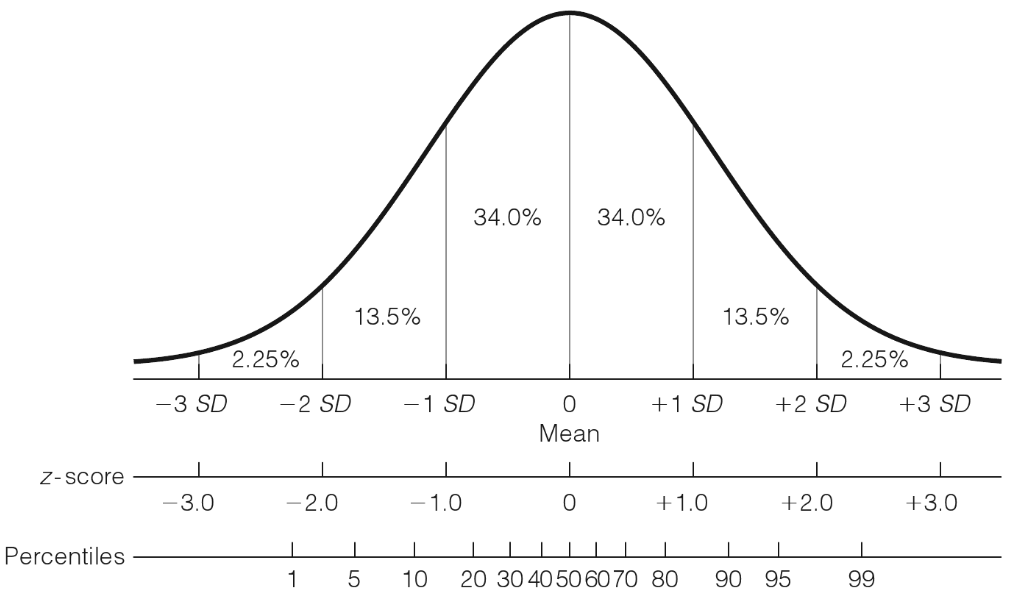
\includegraphics[scale=0.4]{zscore}}
\end{figure}

\section{K Nearest Neighbours (KNN)}
\label{sec:knnExplanation}
KNN \cite{knn} is a straightforward classification technique, in which given an input it is able to classify it to a certain class. As the name implies it takes the closest K neighbours and depending on the majority of their classes it determines the class of the input. Figure \ref{fig:knn} demonstrates KNN ($K=3$) while classifying X using a data set containing 3 different classes. In this case, input X is classified as Red due to the fact that the majority of its 3 closest neighbours are Red.
\begin{figure}[H]
\caption{At KNN=3, Input X is classified as Red}
\label{fig:knn}
\centerline{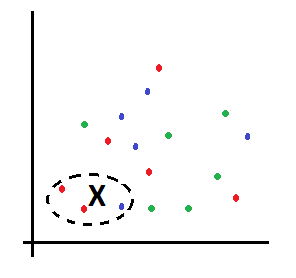
\includegraphics[scale=1]{knn}}
\end{figure}

\chapter{Literature Review}
\section{Introduction}
In this chapter, we describe the studies and research works that have been carried out in the field of energy-efficient sensor networks. Additionally, we shall delve into other areas such as predictive analytics and edge computing. We then evaluate the other works whilst comparing them with our approach.

\section{Wireless Sensor Networks}
A.Manjeshwar et al. \cite{teen} describe how WSNs are usually unattended and need to be fault-tolerant so the need for maintenance is minimized. This is desirable as in most cases these sensors are deployed in inhospitable terrain and are inaccessible. They developed a network model called TEEN to tackle the power availability and network routing issues so as to increase fault tolerance. Figure \ref{fig:teen} shows an example of their network made up of several clusters. Nodes inside the cluster send data only to their cluster-head, which saves energy. Data is sent only if certain thresholds are met. Cluster-heads are changed so as to not drain the energy of one node, which requires additional cost to re-calculate thresholds and dissemination of new meta-data. The biggest disadvantage is the dependency on the thresholds, since if they are not met data is never sent.

\begin{figure}[H]
\caption{Hierarchical Clustering \cite{teen}}
\label{fig:teen}
\centerline{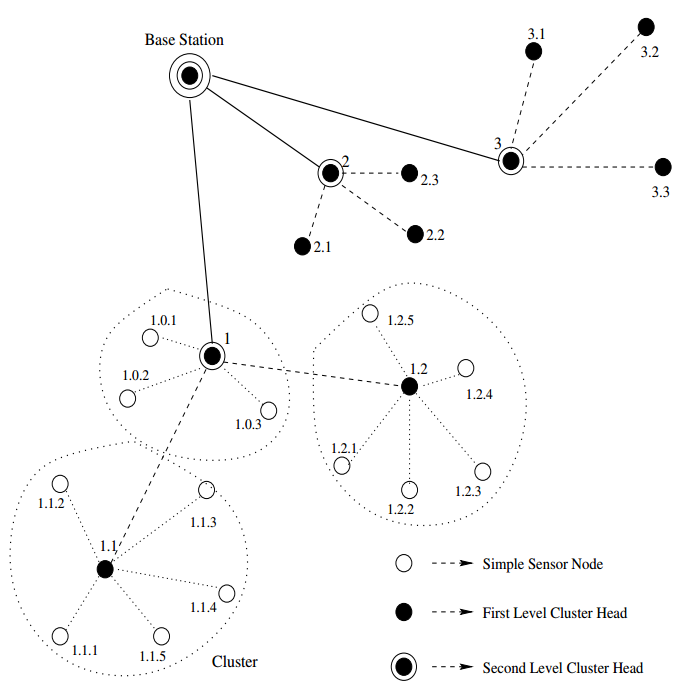
\includegraphics[scale=0.5]{teen}}
\end{figure}

Another protocol called SPIN \cite{adaptiveProtocols} deals with information dissemination in wireless sensor networks. It is short for Sensor Protocols for Information via Negotiation. It uses application knowledge about the data to construct meta-data and then transmit this meta-data instead. The main constraint of this approach is that the meta-data has to be shorter than the actual data so as to achieve network efficiency. The disadvantage is that this approach is very application specific and might achieve the same efficiency for all use cases. In fact, there is no formal definition of what the meta-data consists of. The interesting part of this approach is that it uses 3 types of messages to communicate between nodes with the intent of sharing knowledge and make informed decisions on resource management.

Similar to our work is Adaptive Data Forwarding (ADF) \cite{adaptiveDataForwarding} developed by C. Anagnostopoulos. It considers devices with limited computing resources capable of building local models which then decide whether message transmission is required or not. The main objective of this approach is to achieve a balance between energy consumption and error propagation. We shall go a step further by extending this model and study the analytics perspective. The model in \cite{timeOptimizedContextual} deals with mobile context-aware systems. Their purpose is to disseminate information about the surrounding environment between each other. They assume that the information is delay tolerant and use the Optimal Stopping Theory (OST) to decide whether messages should be sent or not. Delaying the transmission of a message incurs an error penalty and OST allows for the system to approach the maximum allowed error penalty without ever surpassing it. In our system, we will allow for a fixed error and won't delay messages as we are interested in comparing the error allowance with the query accuracy at the concentrator level.

R.Shah, developed an Energy Aware Routing protocol \cite{energyAwareRouting} for sensor networks with network longevity in mind. This is similar to what we are trying to achieve, which is an efficient network that does not waste resources. They approach the problem from a different perspective as they are interested from where data is routed between nodes. They argue that if data is always routed through the path which consumes the least energy, then these nodes will deplete their battery first. Their protocol uses different paths so as to maximise the survivability of the network. The Directed Diffusion \cite{directedDiffusion} system proposed by C.Intanagonwiwat uses a similar concept to exploit empirically good paths and achieve energy efficiency. Our approach tries to increase network efficiency by decreasing the actual amount of messages sent.

C. Tung Chou \cite{informationCollection} approaches this problem by using adaptive sensing. This model assumes synchronization between nodes and is very computationally complex. The computational calculations are not considered in the model evaluation, although it affects the results. Moreover, the model makes assumptions on the sensed data. In our model, we do not make these assumptions as we do not know the distribution of the sensed data. The authors in \cite{energyEfficientDataManagement} propose an energy efficient data management model which is based on routing and data aggregation. The disadvantage of this model is that it requires training to construct the routing tables. This would incur a substantial amount of computational effort which is not taken into account when evaluating the model. They also make an assumption on how the sensor nodes are distributed and the number of sensor nodes that make up the network. In our model, we will not be making any assumptions on the structure of the network. R. Arroyo-Valles \cite{optimalSelective} propose an optimal Selective Transmission protocol for energy efficient distribution of knowledge between nodes. Information is transmitted only when the message is statistically important based on the statistical distribution, energy costs, and available battery. This computation incurs extra energy cost but is not considered.

\section{Edge Computing}
Edge computing extends the cloud computing paradigm to the edge of the network. This enables a new brand of applications and services. Our system will be using this concept to place some computational logic inside the sensors, away from the concentrators. F. Bonomi et.al \cite{fogComputing} describe edge computing as a large number of nodes geographically distributed with mobility support. It must support real-time interactions, wireless access, and heterogeneity. Furthermore, on-line analytics are an essential component due to the context awareness edge computing is capable of providing. 

M. Rabinovich and Z.Xiao \cite{replicatingInternetApplications} describe an Application content delivery network based on edge computing. They produce a middleware platform for providing scalable access to Web applications. Currently, edge computing is being promoted as a strategy to achieve highly available and scalable Web services. \cite{authenticatingQueries} We shall extend this concept to wireless sensor networks and enable the data of each sensor to be accessible from concentrators while at the same time maximising network efficiency.

\iffalse
\section{Predictive Analytics}
\cite{EdgePowerConsumptionManufacturing}
\cite{efficientPredictiveAnalytics}
\fi

\chapter{Contributions}
In this chapter, we discuss our major contributions with the aim of improving WSNs. More specifically how we can increase network efficiency, which extends the devices' life time. We shall delineate a strategy for extracting knowledge from the raw context, by locally learning the context in real-time using on-line multivariate stochastic gradient descent. Based on this knowledge, we then decide whether it is worth it to transmit data or not.
Additionally, we look into how we can minimize the error when querying the knowledge found inside the concentrators.

\section{Model Description}
We start by considering an IOT system composed of multiple sensor nodes and a concentrator depicted in figure \ref{fig:sn}. Sensor nodes are only capable of communicating with concentrators. Concentrators can then be queried or in turn be considered as sensor nodes and connected to a larger tree structure, creating a larger more complex network. Resources are reserved for communication, processing and data sensing. Message transmission consumes much more energy when compared to the processing and data sensing tasks. \cite{teen} Thus, we argue that if the nodes continuously sense data and only transmit this information when it is essential, we could create a more energy efficient network. A.Manjeshwar et al. \cite{teen} states that this is possible because sensor networks are "data-centric", meaning that data is requested based on certain attributes and not requested for a certain node. The requirements of each WSN change according to the application, as some nodes might be static while others mobile. When nodes are adjacent to each other certain similarity might occur, thus, data can be aggregated. A common query in these systems is for example which area has humidity $<$ 10\% rather than what is the humidity of area $X$. We can use this knowledge to our advantage and define a system that can minimize the number of messages transmitted while at the same time still provide accurate results from queries.

\begin{figure}[H]
\caption{Model Example}
\label{fig:sn}
\centerline{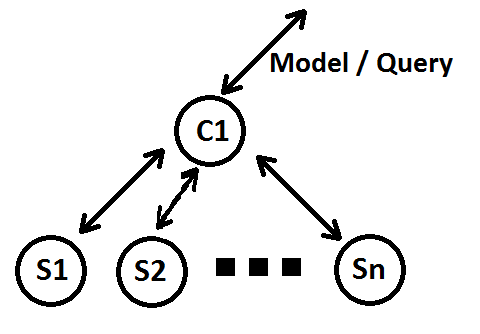
\includegraphics[scale=0.5]{sensornetwork}}
\end{figure}

\section{Network Efficiency}
Consider a sensor node $i$ which receives a new data item $p(t)$ at time $t$. Our system needs to decide whether it is worth transmitting this new data or not. To achieve this, we create a local model based on linear regression. The function we compute will enable us to predict the error and have a quantifiable way of deciding whether transmitting $p(t)$ is worth it or not. Since each sensor node has limited resources, both computational and storage limitations we use on-line stochastic gradient descent to calculate the regression line. A full detailed description of on-line stochastic gradient descent can be found in the Preliminaries chapter, section \ref{linearregression}. Using this algorithm we avoid storing a history of values and instead we consider each new data item alone, then discard it. 

Each sensor $i$ locally and incrementally builds its own model from sensing the pairs $(x,y)$. After a period of learning, each sensor sends its model parameters to a centralized concentrator. Take for instance weights $w=[w_0,w_1,w_2]$ from equation \ref{eq:modelParams}. 

\begin{equation}
\label{eq:modelParams}
f[i](x) = w_0 + w_1x_1 + w_2x_2
\end{equation}

Once a sensor $i$ has sent its local model $F[i](x)$ to the concentrator, then for every new $(x,y)$ data pair it receives, it is capable of updating the local model and deciding whether to update the concentrator model as well. For every new $(x,y)$ the $w$ parameters might change when compared to the original model sent previously to the concentrator. Sensor $i$ upon receiving an $(x,y)$ pair it updates the local model and predicts the output $y*$ from its current local $f[i](x)$ with parameters $w'$ and then measures locally the error $e* = |y-y*|$. If the model has not significantly changed the 'obsolete' model in the concentrator will experience a similar error. Sensor $i$ keeps a copy of the original w (obsolete model in concentrator), thus, knows exactly the error the concentrator would experience. Hence, let us denote this error from the original local model as $e\# = |y - y\#|$ where $y\#$ is the prediction of y when involving the original (obsolete) model $f[i](x)$ with parameter $w$. At that time, sensor $i$ has two prediction errors: $e*$ and $e\#$. The $e\#$ is the error that concentrator would experience if the same input $x$ was used.

\begin{equation}
\label{eq:differenceError}
\delta = |e* - e\#|
\end{equation}

Using Equation \ref{eq:differenceError} we are able to get the discrepancy in error between the 2 models. We then use the condition $\delta > THETA$ to determine whether it is worth it to update the obsolete model or not. A $THETA=0$ would mean that the local and concentrator model would be synchronized at all times. On the other hand, when we increase $THETA$ we transmit fewer messages, thus, increase network efficiency. This would also mean we are now susceptible to an increase in error between the 2 models. Figure \ref{fig:nea} shows a simplified flowchart of the algorithm just described in this section.


\begin{figure}[H]
\caption{Sensor Node Flowchart}
\label{fig:nea}
\centerline{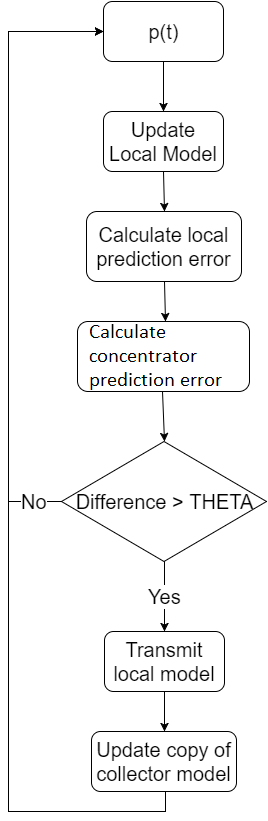
\includegraphics[scale=0.7]{NetworkEfficiencyAlgorithm}}
\end{figure}

\section{Ensemble Learning}
\label{sec:ensembleLearning}
The previous section explained our algorithm which increases network efficiency by transmitting fewer messages to the concentrator. This is done by altering $THETA$ which determines the acceptable error. An increase in network efficiency means that sensors working on battery power can last longer without the need of recharging. As previously mentioned the purpose of an IOT system is that it can be queried from the "root" (concentrator). In this section, we aim to extend the model defined in the previous section to reduce the error at the concentrator level.

Naively the concentrator would have all the $(x,y)$ data pairs and when queried with an arbitrary $x$, it can directly search in its storage for the best match and return $y$ accordingly. In our model the concentrator collects a function $f[i](x)$ for each sensor $i$ which simulates the data collected. The ideal scenario is that when the concentrator receives query $x$, it would also know which function $f$ it should use to predict $y$. Unfortunately, in a real-life scenario, this is not possible as we would not know to which sensor $x$ is related to.

One solution is that the concentrator proceeds with averaging the prediction results from all the collected functions $f[i](x)$. The concept behind averaging all the predictions ensures that the over-estimates and under-estimates are balanced out. We argue that this might not always produce an optimal result and it can further be improved. There exist scenarios where an input $x$ is not observed by some of the functions, thus, leading to poor predictions. Take for instance the case where multiple thermometers are sparsely placed around a building. Sensors next to a kitchen might, in general, observe temperature readings in a higher range than sensors placed outside. Given a high temperature $x$, would it be better to average the predictions from all the sensors or use only the kitchen sensors?

With this concept in mind, we extend the previous model and add data representatives of the input space. Using these data representatives, the system would be able to determine whether a function $f$ is familiar to the query $x$ or not. To elect data representatives we use an on-line clustering algorithm which quantizes the input space. We implemented both K-Means and ART which are described in detail in the Preliminaries chapter; section \ref{sec:knnExplanation} and \ref{sec:artExplanation}. When a data pair $(x,y)$ is used to update the model, we also update the centroids in the clustering algorithm. The centroids are transmitted to the concentrator along with the local model. Figure \ref{fig:clusters53knn} shows the quantized input space of 5 sensors using 3 Clusters for each sensor.

\begin{figure}[H]
\caption{Depicting the quantized input space $x_0,x_1$ of 5 sensors ($K=3$)}
\label{fig:clusters53knn}
\centerline{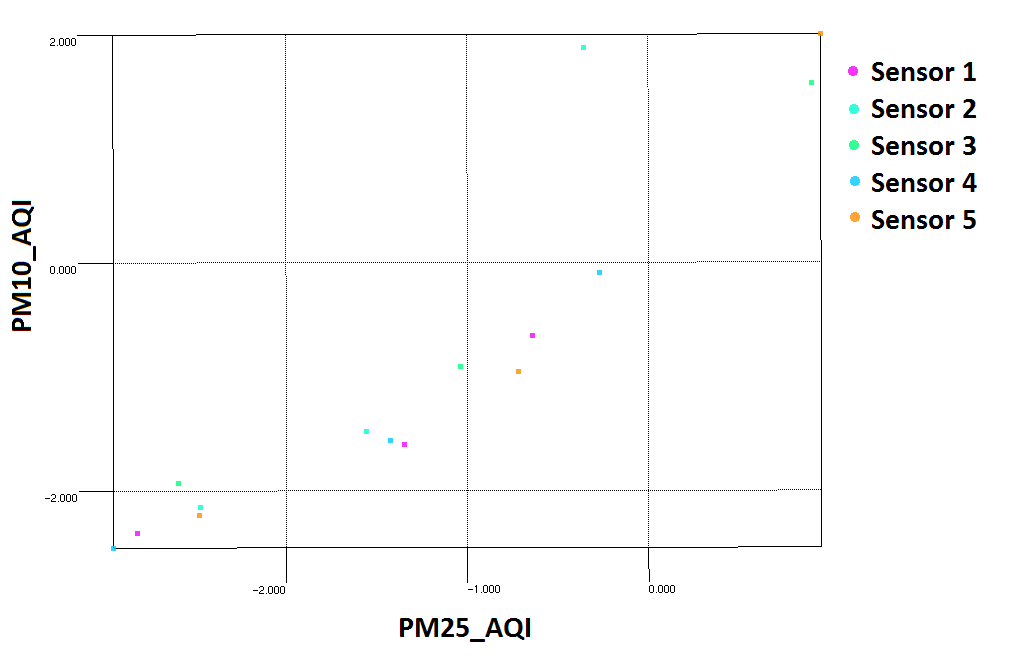
\includegraphics[scale=0.7]{clusters5sensors3knn}}
\end{figure}

The concentrator now has the necessary information to determine what the input space of each function is. When query $x$ is submitted, the concentrator can select the functions which have data representatives in the vicinity. The assumption is that these functions were generated from values similar to the query, thus, have more reliable knowledge.

\section{Adding the "Reliability" variable}
\label{sec:reliabilityVariable}
Using on-line clustering the concentrator is able to select which functions to use based on the distance between query $x$ and centroids. We believe the distance alone might not be sufficient enough to describe the input space of each function. Our intuition is that some sensors produce more accurate results than others. To study this, we performed an analysis on the Beijing Air Quality dataset \cite{air-quality-inference-meets-big-data} and trained a regression model for each sensor. We then isolated 2 sensors at a time and predicted $y$ using 3 different methods; 

\begin{itemize}  
\item Endogenous error - In this test we predict $y$ of sensor $i$ using regression function $f(i)$.
\item Exogenous error - In this test we predict $y$ of sensor $i$ using regression function $f(i+1)$.
\item Fusion error - In this test we predict $y$ of sensor $i$ using both regression functions $f(i)$ and $f(i+1)$ and then take the mean.
\end{itemize}

\begin{figure}[H]
\caption{Endogenous, Exogenous, Fusion errors}
\label{fig:functionsErrors}
\centerline{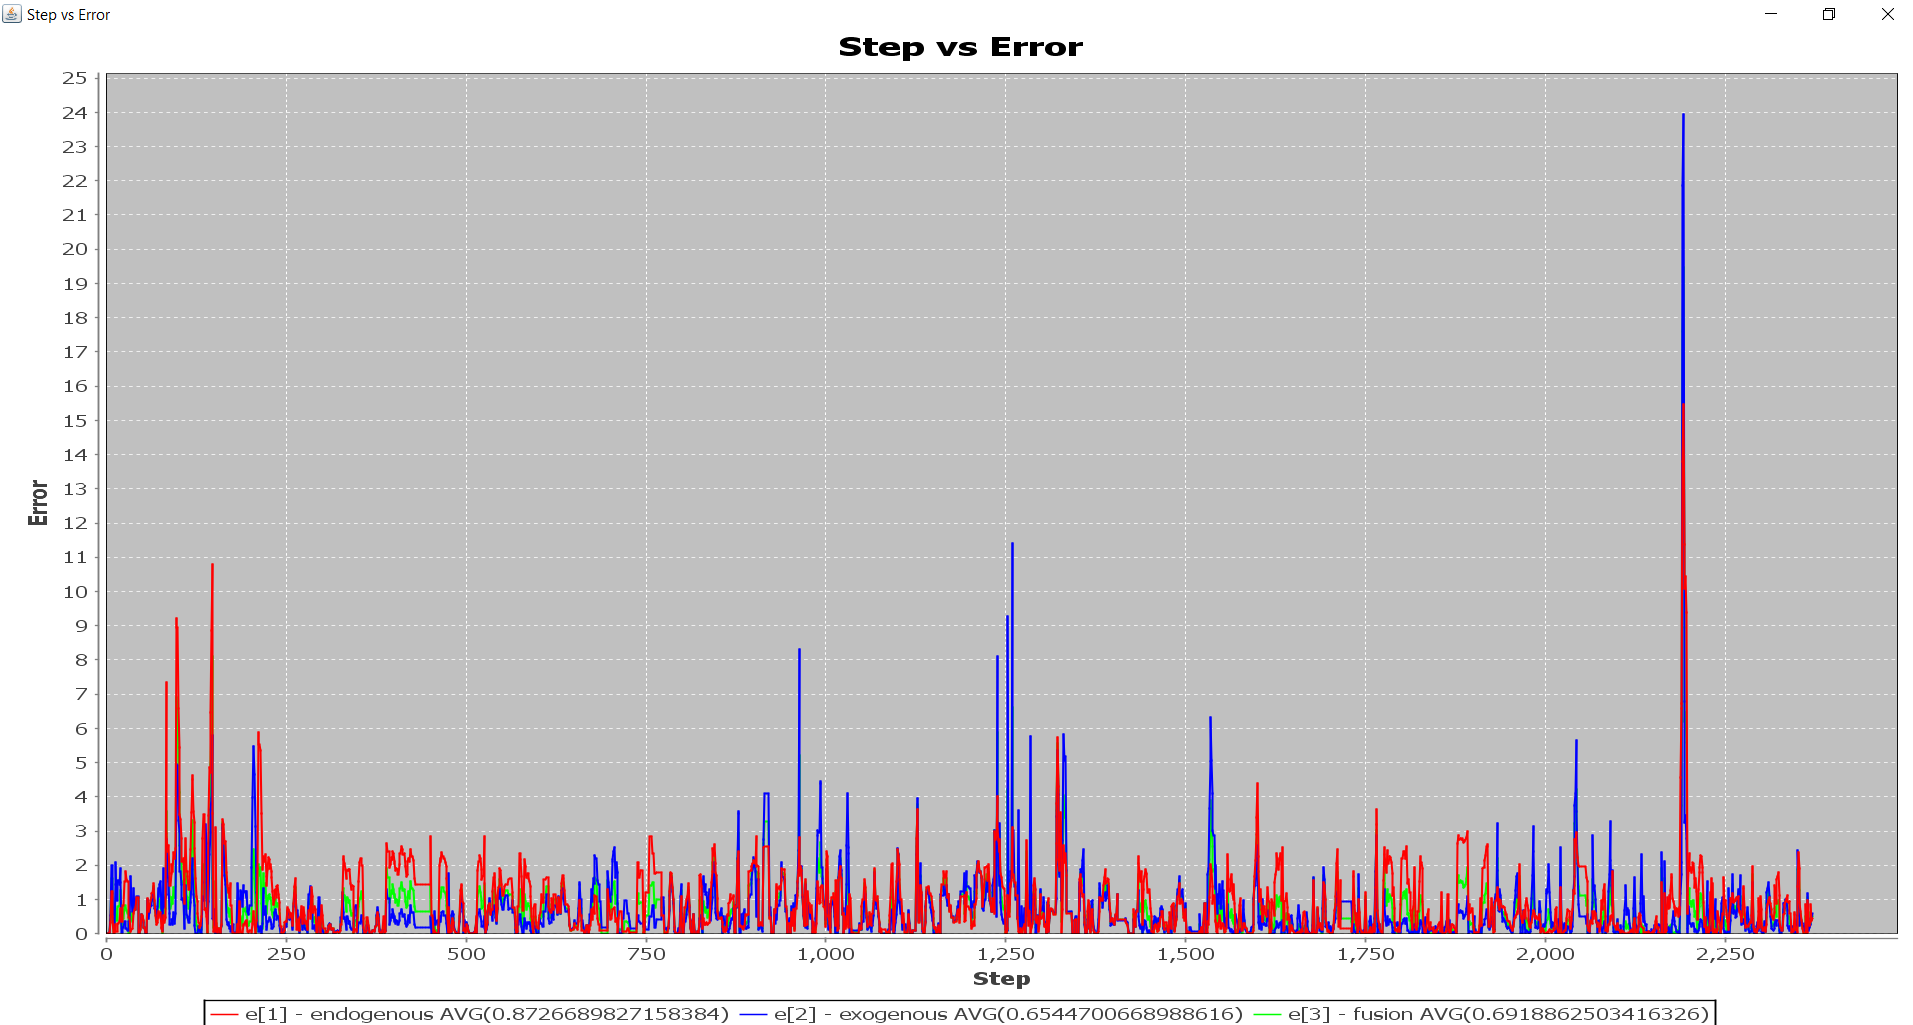
\includegraphics[scale=0.4]{e1e2e3}}
\end{figure}

Figure \ref{fig:functionsErrors} shows one of the studies done using the first 2 sensors. In this case, using just the regression model from another sensor (exogenous) was more accurate than using its own model. The reason might be because some centroids are more popular (more experienced), while others yield less error in certain situations. This is where ensemble learning is useful, and we can leverage the knowledge the concentrator has about every sensor attached to it. The concentrator should try to choose a subset from all the sensors to provide more accurate results. Centroids which are frequently updated tend to have a higher average error due to the frequent updates to the regression model. Hence, we should consider the number of times each centroid is used to determine the popularity. Thus, along with each centroid, we include an error value and the number of times used.

\begin{equation}
\label{eq:ourEquation}
weight=\frac{e^{-distance} + e^{-error} + used}{3}
\end{equation}

\begin{figure}[H]
\caption{$e^{-x}$ Function}
\label{fig:e-x}
\centerline{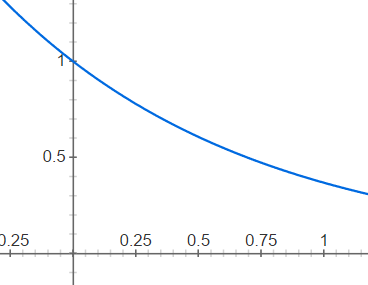
\includegraphics[scale=0.6]{e-x}}
\end{figure}

Equation \ref{eq:ourEquation} defines how we assign a weight to each centroid in relation to a given query. Once we sort the centroids in descending order according to their weight, we would get an amalgamation of the 3 properties; closest, lowest error and most popular. Note, that the \textit{distance} and \textit{error} values are normalized between 0 and 1 so as to makes use of the exponent function shown in figure \ref{fig:e-x}. As distance and error approach 1 (highest possible due to normalization), the exponent function inverts them and gives them a low value. On the other hand as \textit{used} approaches 1 we would like to give it a higher weight, thus we leave it as is.

\section{Summary}
In this chapter, we first explained the statistical mechanism which allows knowledge distribution in a network efficient manner. Secondly, we extended this mechanism to include information about the input space for each sensor. With this added information the concentrator is able to intelligently select which subset of models to choose depending on the query.

\chapter{Design and Implementation}
In the previous chapter we laid the theoretical groundwork and intuitions of our system, and now we proceed to examine how they were implemented into a fully functional system. We begin by explaining the dataset that we used and how it is structured as it will affect the design of the system. Afterwards, we explain how we implemented a system capable of simulating an IoT environment, including the network aspect and statistics gathering. We then explain in detail our contributions regarding network efficiency and ensemble learning mentioned in the previous chapter.

\section{Dataset}
We will be using the air quality data \cite{air-quality-inference-meets-big-data} collected from air quality monitoring stations in Beijing. There are 36 independent sensors which can be considered as our IoT devices. All of these devices will need to transmit the knowledge to the concentrator. We chose 3 fields from the dataset and verified there was a correlation among them. Let $x_1$ be \texttt{PM25\_AQI}, and $x_2$ be \texttt{PM10\_AQI}. These values represent the concentration levels of fine particulate matter (air pollutant) with an aerodynamic diameter of less than 2.5, 1.0 respectively. We will consider $y$ as the \texttt{NO2\_AQI} which represents the concentration levels of Nitrogen Dioxide. These gases are emitted by all combustion processes and have a negative impact on human life, example Nitrogen dioxide is linked with the summer smog. \cite{Richter2005}

We normalize the data using the standard score as explained in the Preliminaries chapter. The normalized $x_0,x_1,y$ will be used during the implementation and evaluation phases. Figure \ref{fig:dataset} displays the whole normalized dataset with a general linear regression model amalgamating all the sensors together.

\begin{figure}[H]
\caption{3D graph plot of dataset along with general linear model}
\label{fig:dataset}
\centerline{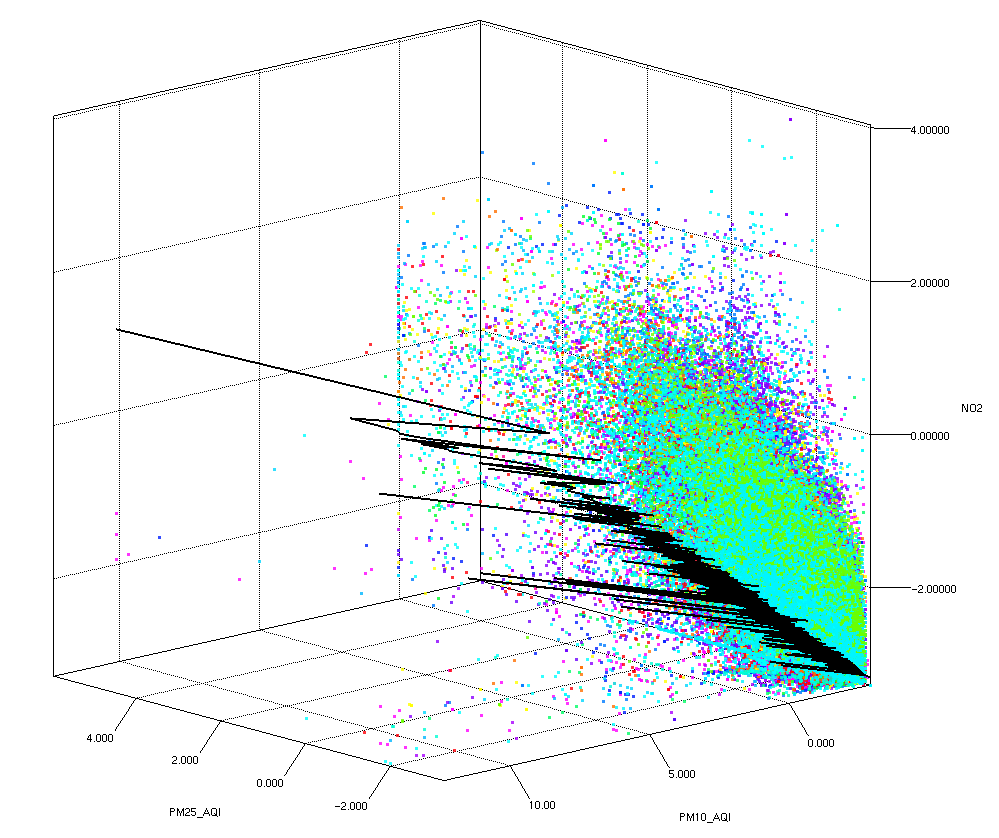
\includegraphics[scale=0.6]{dataset}}
\end{figure}

\section{Decentralized Learning with Reliability}
We first started by creating a list of requirements of the system and then designed the system's components around it. We needed to simulate multiple sensors reading information at unpredictable times. This information had to be made accessible through a concentrator for querying. Additionally, we needed to gather statistics so as to be able to analyze the performance and compare different simulations. We decided to us Java to implement the simulator as it felt very intuitive to read the data into multiple threads, add our contributions and analyze them.

A \texttt{SensorManager} class was created that handles the reading of new information from the dataset for each sensor. A \texttt{Sensor} thread is then initiated for each sensor. Each sensor reads data from the \texttt{SensorManager} and stores a local model $f'(x)$ and a copy of the concentrator model $f(x)$. When a new data item is read, $f'(x)$ is updated and the closest cluster determined. After the local and concentrator errors are calculated, an error is associated with the closest cluster so as to have the notion of a reliability factor as explained in the contributions chapter. Lastly, the algorithm checks the discrepancy between local and concentrator errors, and if it is larger than $THETA$ is transmits the local knowledge to the concentrator. This procedure is formally described in algorithm \ref{alg:talg}. Algorithm \ref{alg:talg} is the full implementation of all the contributions described in the previous chapter. 

\begin{algorithm}[H]
$w'=(w'_0,w'_1,w'_2)$ (local weights)\;
$w=(w_0,w_1,w_2)$ (concentrator weights)\;
$f' = w'$ (local model)\;
$f = w$ (concentrator model)\;
$centroids$ = create centroids list\;
 \While{data is available}{
  $x_1,x_2,y = p(t)$ (read from sensor)\;
  update $w'$ of $f'$ model using $x_1,x_2,y$\;
  $c$ = closest centroid to $x_1,x_2$ from $centroids$\;
  \If{learning phase finished}{
   $Y' = f'(x_1,x_2)$\;
   $Y = f(x_1,x_2)$\;
   $e' = (Y'- y)^2$ (local error)\;
   $e = (Y - y)^2$ (concentrator error)\;
   associate $e'$ to $centroids[c]$\;
  \If{$e > e'$}{
  	$discrepancy = e - e'$\;
  	\If{$discrepancy > THETA$}{
  		Transmit $w'$,$centroids$ (and error associated with each centroid)\; 
  		$f$ = $f'$\;
  	}
  }
 }
 }
 \caption{Transmission algorithm}
 \label{alg:talg}
\end{algorithm}

\section{Query Analytics}
\label{sec:queryAnalytics}
The \texttt{Concentrator} class is tasked with continuously receiving local models in no particular order and storing them. Furthermore, the concentrator needs to make its knowledge available for querying. Thus, we expose several methods which allow querying using different algorithms. This allows us to take measurements and then evaluate them to determine which gives the minimum error. 

\subsection{Average}
Algorithm \ref{alg:avgModels} is the naive approach which predicts $y'$ using all the models and then calculates the mean.

\begin{algorithm}[H]
 query\ = $x_1,x_2$\; 
 $f$ = List of sensor models\;
 $y'=0$\;
 \ForEach{f[i]}{
 	$y' += f[i](x_1,x_2)$\;
 }
 calculate mean $y'$
 \caption{Averaging models}
 \label{alg:avgModels}
\end{algorithm}

\subsection{KNN - Distance}
Algorithm \ref{alg:closestModels} uses the centroids to calculate the distance between the query and each centroid. Then the nodes are sorted by distance in ascending order and the first $K$ models are used to predict $y'$. The concept is that we only use the functions which "are built from that quantized space". This should skip the outliers and return a more accurate result when compared to the naive approach (algorithm \ref{alg:avgModels}).

\begin{algorithm}[H]
 query\ = $x_1,x_2$\;
 $f$ = List of sensor models\;
 $centroids$ = list of centroids\;
 $distances$ = list of distances\;
 \ForEach{$centroids[i]$}{
 	$distances[i] = distance(query,centroids[i])$\;
 }
 sort $distances$ ascending\;
 $y'=0$\;
 \For{int i=0; i $<$ K; i++}{
 	$y' += f[distances[i].nodeId](x_1,x_2)$\;
 }
 calculate mean $y'$\;
 \caption{Closest K nodes}
 \label{alg:closestModels}
\end{algorithm}

\subsection{KNN - Reliability}
Algorithm \ref{alg:reliableModels} is an extension of algorithm \ref{alg:closestModels}. Rather than considering only the distance from the query we try to materialize a "reliability" factor. With each centroid, we store an error value and the number of times the centroid was used. This information is then used to calculate the weight. The equation is explained in detail in the contributions chapter; section \ref{sec:reliabilityVariable}. A low \texttt{error}, low \texttt{distance}, and a large \texttt{used} value would  result in large weight. Thus, we sort the weight in descending order and choose the first $K$ models. We also normalize the first $K$ weights so as to adjust the predicted value accordingly. The first $K$ models should be the most reliable and give us a more accurate result when compared to algorithm \ref{alg:closestModels}.

\begin{algorithm}[H]
 query\ = $x_1,x_2$\;
 $f$ = List of sensor models\;
 $centroids$ = list of centroids\;
 $errors$ = list of errors\;
 $used$ = list of times used\;
 $weights$ = list of weights\;
 \ForEach{$centroids[i]$}{
 	$d = distance(query,centroids[i])$\;
 	$err = errors[i]$\;
 	$u = used[i]$\;
 	$weights[i] = \frac{e^{-d} + e^{-err} + u}{3}$\;
 }
 sort $weights$ descending\;
 $normalizedWeights$ = normalize first K $weights$\;
 $y'=0$\;
 \For{int i=0; i $<$ K; i++}{
 	$y' += f[weights[i].nodeId](x_1,x_2) * normalizedWeights[i]$\;
 }
 calculate mean $y'$\;
 \caption{Most reliable K nodes}
 \label{alg:reliableModels}
\end{algorithm}

\section{Statistics Gathering}
Lastly, we needed a way to gather performance statistics for each run configuration. Each class mentioned previously keeps track of various statistics such as messages sent, errors, etc.. The \texttt{QueryPerformer} class was created with the purpose of fulfilling two tasks. Firstly, gathering all the performance statistics in one place and saving it into a readable text file for visualization purposes. Secondly, execute the validation queries at concentrator level to evaluate the accuracy. This class is initialized once all sensors have read the last piece of data and finished running their logic.

\chapter{Evaluation and Case Study}
In the introduction of this report we pointed out the project objectives which were;
\begin{itemize}  
\item The implementation of a system capable of simulating an IoT environment and maximise network efficiency.
\item Intelligent sensors capable of extracting context and decide whether it is worth to transmit this knowledge or delay.
\item Evaluate the query accuracy of our system by comparing it to a naive system which sends data continuously without regarding battery consumption.  
\end{itemize} 
Up to now we presented our algorithms and described the implementation of our system. In this chapter, we evaluate the performance of our system using the Beijing Air Quality data\cite{air-quality-inference-meets-big-data} and comment on the results. This includes the evaluation of both the network efficiency and the query accuracy contribution.

\section{THETA study}
Before measuring the network efficiency we study the effects of altering $THETA$. This is the variable which determines the allowed discrepancy between local and concentrator models. As we increase $THETA$ the number of messages sent drastically decreases but the error between local and concentrator models should increase. This can in fact be seen in the Figures \ref{fig:ThetaMessages} and \ref{fig:ThetaDE}.

\begin{figure}[H]
\caption{$THETA$ vs Messages Sent \%}
\label{fig:ThetaMessages}
\centerline{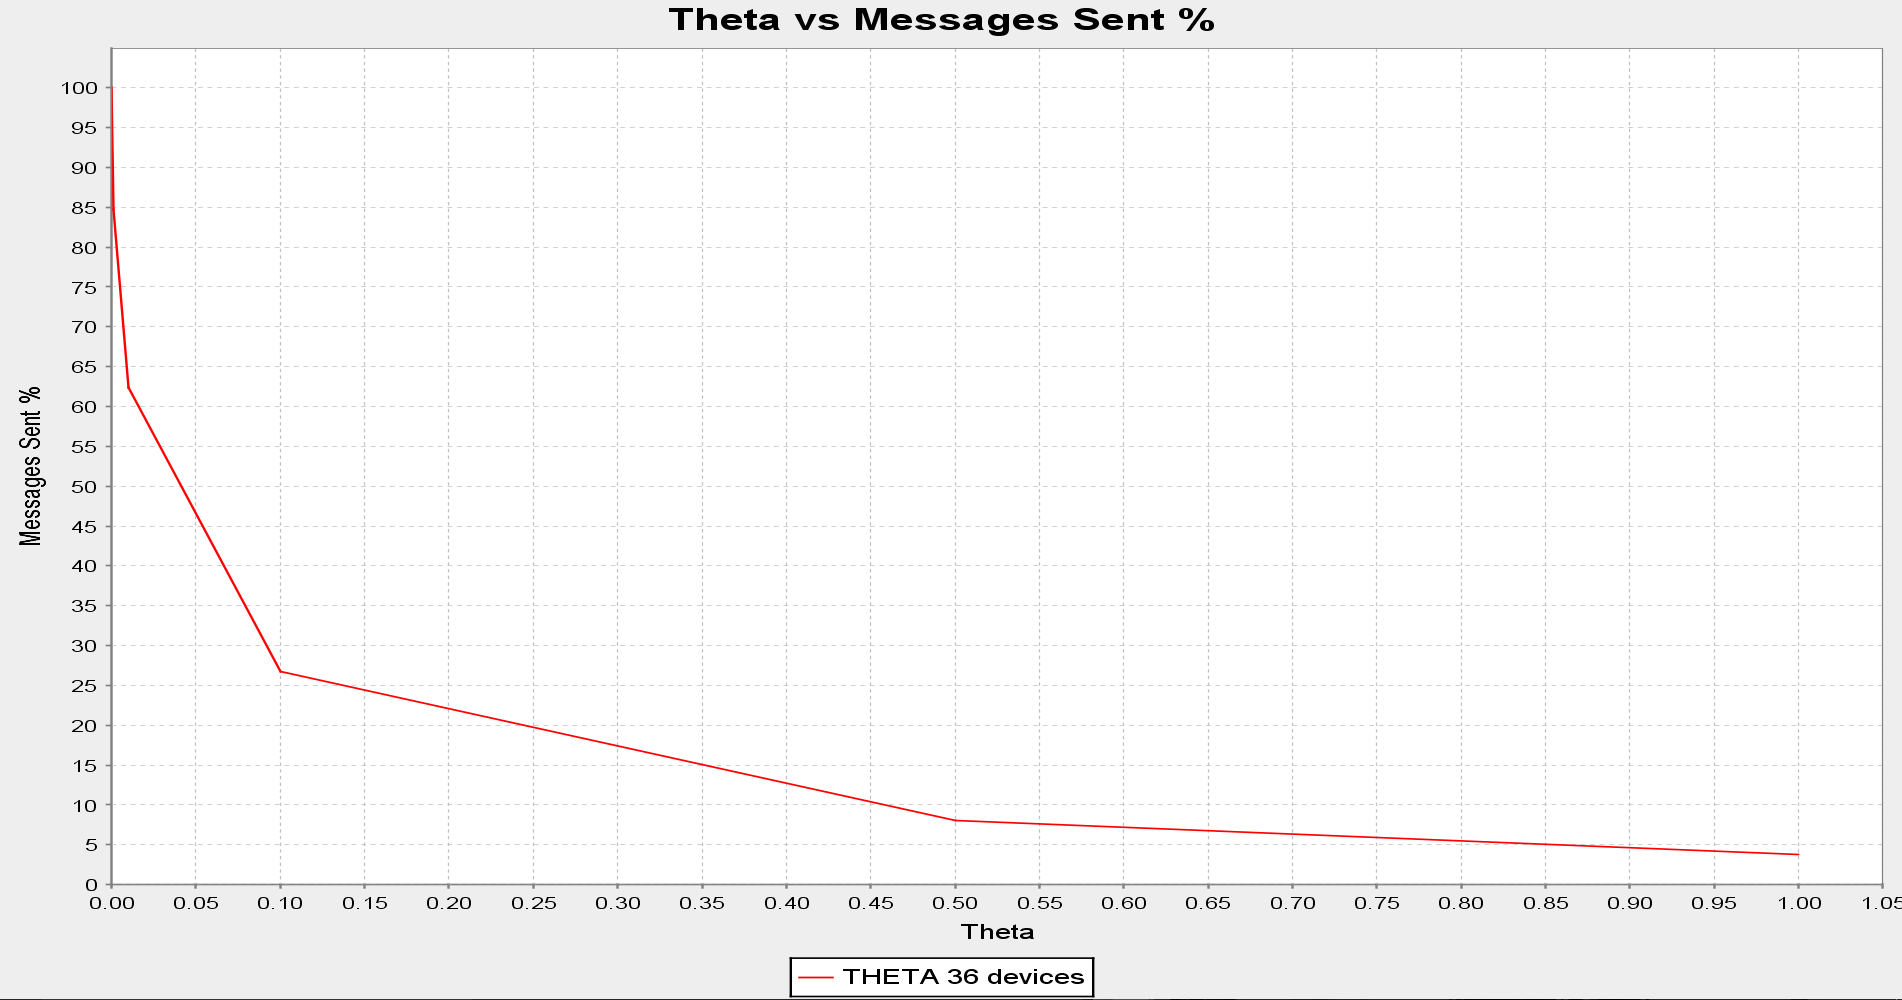
\includegraphics[scale=0.4]{ThetaMessages}}
\end{figure}

\begin{figure}[H]
\caption{$THETA$ vs Difference in Error}
\label{fig:ThetaDE}
\centerline{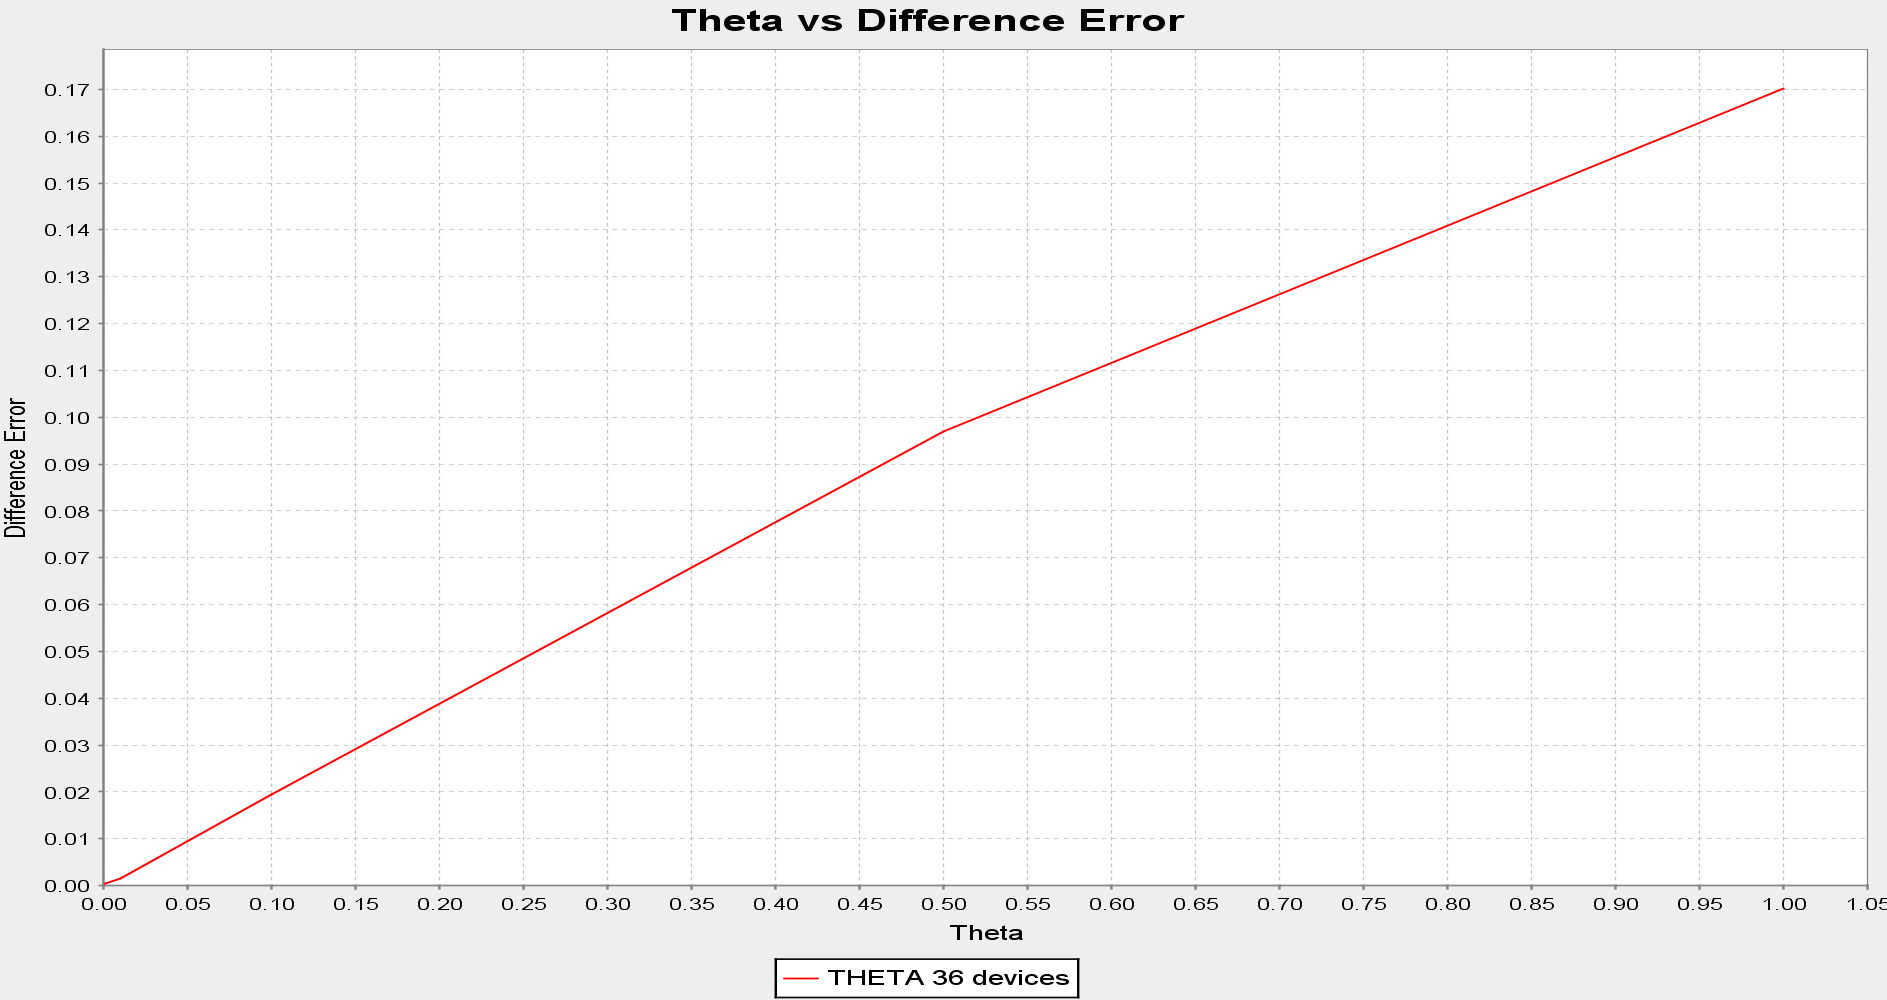
\includegraphics[scale=0.4]{ThetaDE}}
\end{figure}

In figure \ref{fig:MessagesDe} we eliminate $THETA$ and directly study the relationship between \texttt{Messages Sent} and \texttt{Difference in Error}. One notices that there is very minimal difference in error when sending 60\% messages instead of sending all the messages (100\%). This means that around 40\% of the messages have no useful information to the concentrator. The concentrator is able to predict $y$ with the same error rate as the local model. We are capable of measuring the usefulness of messages due to the introduction of a learning model. In this chapter; section \ref{sec:networkefficiency} we use a real case study in which we exploit our algorithm to evaluate the effect of transmitting fewer messages on the devices' battery life.

\begin{figure}[H]
\caption{Messages Sent \% vs Difference in Error}
\label{fig:MessagesDe}
\centerline{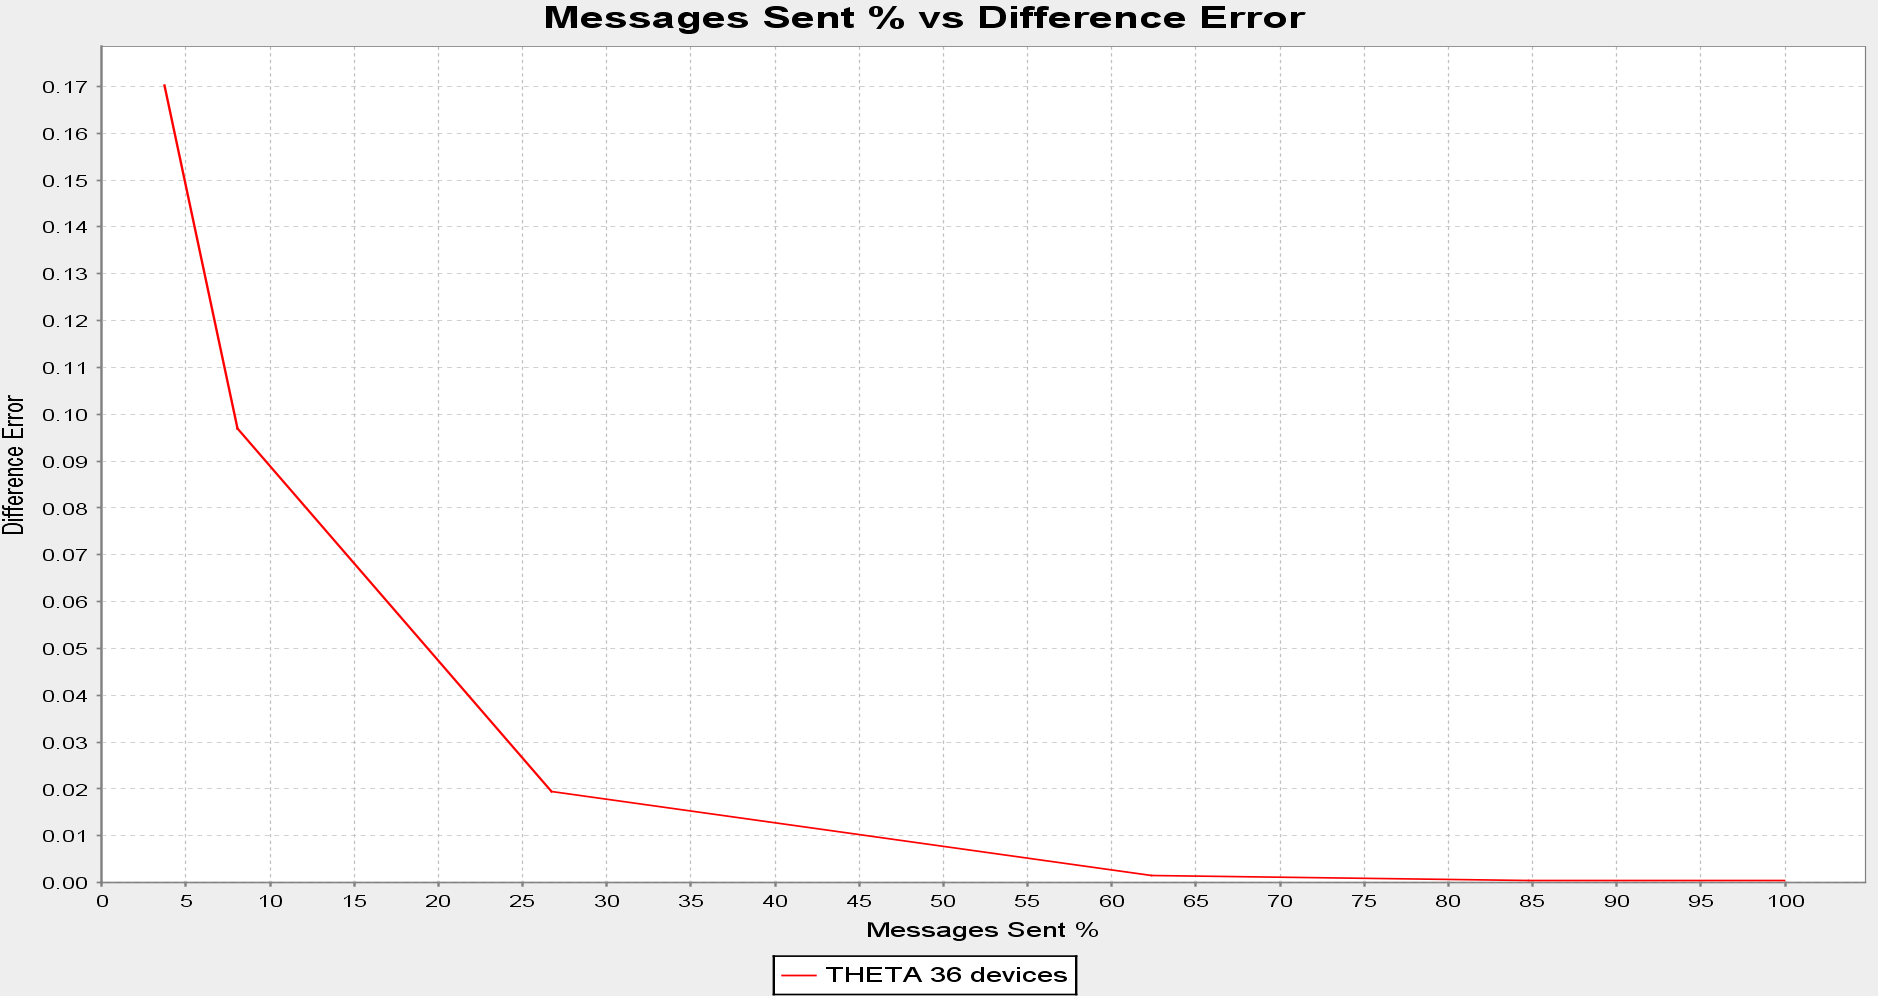
\includegraphics[scale=0.4]{MessagesDe}}
\end{figure}

Furthermore, we stored the number of times the local model was better than the central model for each $THETA$. This is shown in figure \ref{fig:thetaP}. $P$ is the probability that the local model is better than the central model. It is interesting to note that as $THETA$ is increased, the probability that the local model performs better decreases. We believe that this is because as $THETA$ increases the central model is updated less frequently, thus, encapsulating a certain level of generality. This is interesting as it might open up future work regarding whether it would be worthwhile to predict results from a history of models.

\begin{figure}[H]
\caption{$THETA$ vs $P$}
\label{fig:thetaP}
\centerline{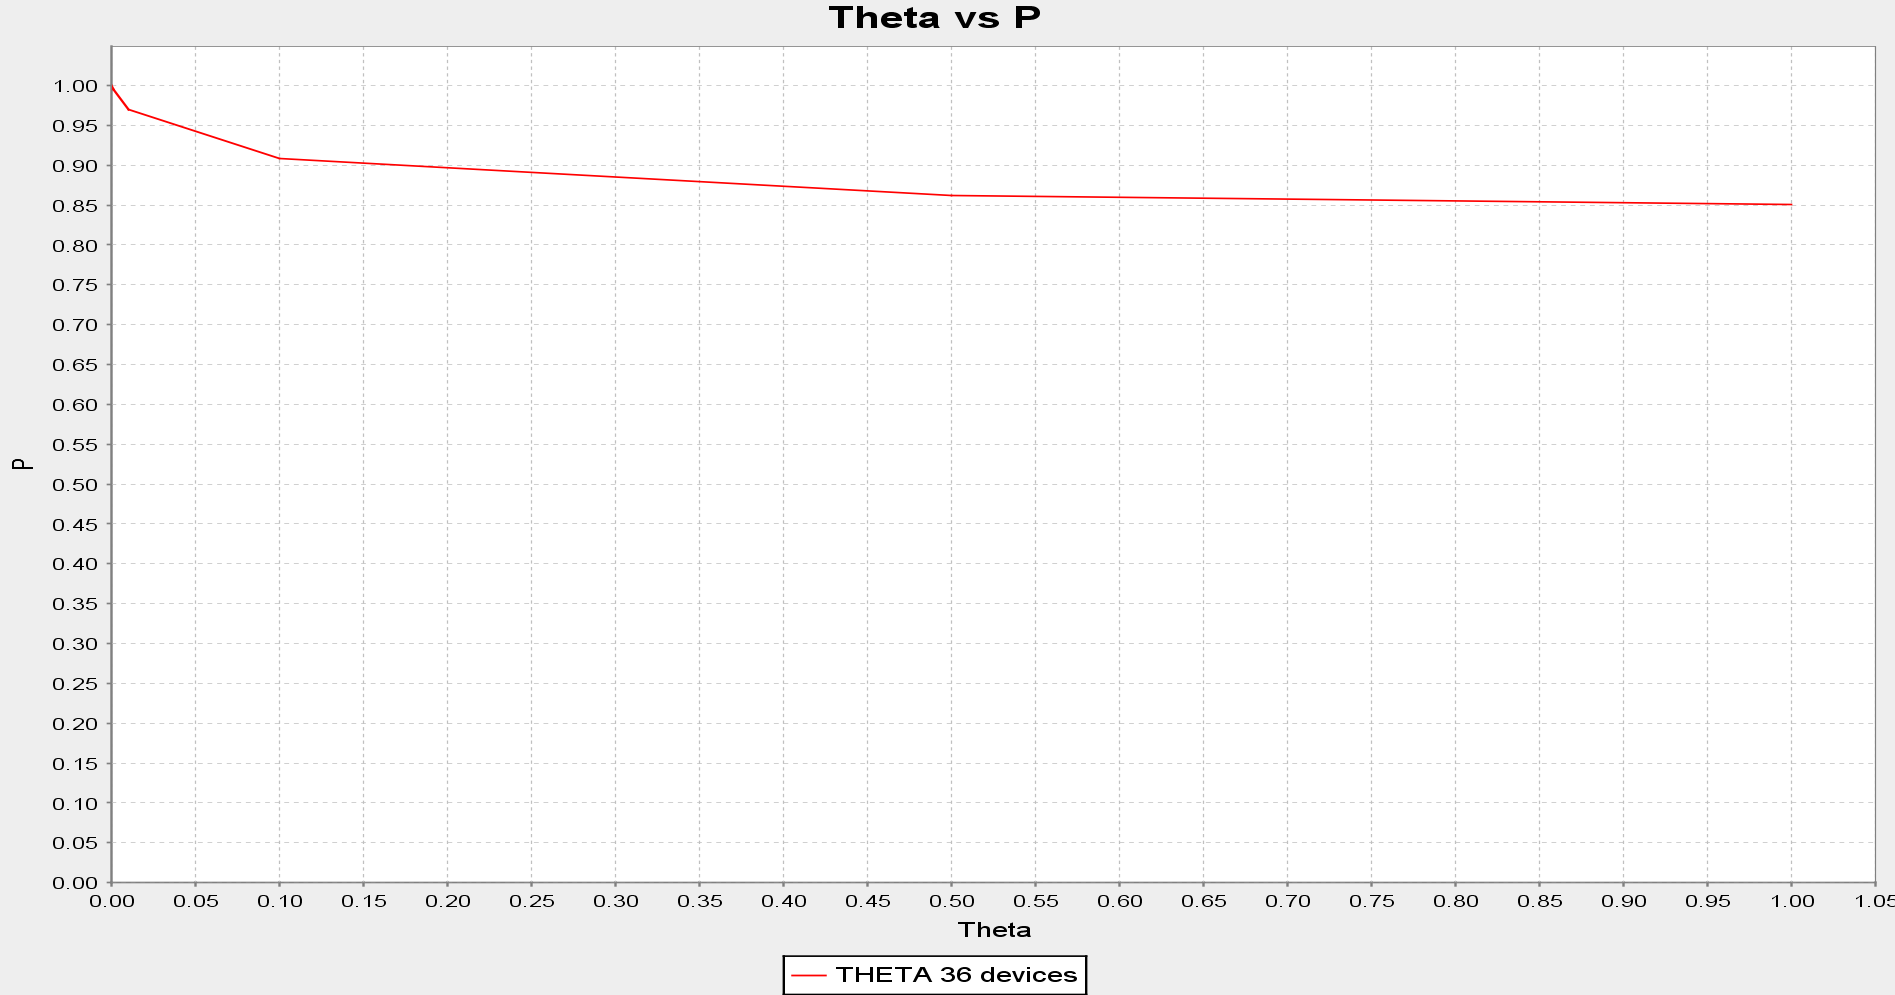
\includegraphics[scale=0.3]{thetaP}}
\end{figure}

\subsection{Probability Density Functions}
Additionally, we measured the mean and variance of the error using an on-line algorithm described in the Preliminaries chapter; section \ref{sec:meanvariance}. The mean and variance allow us to plot the probability density function which is also described in the Preliminaries chapter. This visually shows the likelihood of a certain random variable taking a given value. In our case, the value with the highest likelihood is 0 since we used the standard score normalization.

\begin{figure}[H]
  \caption{Local Model PDF (Error $e'$)}
  \label{fig:thetaedash}
\centerline{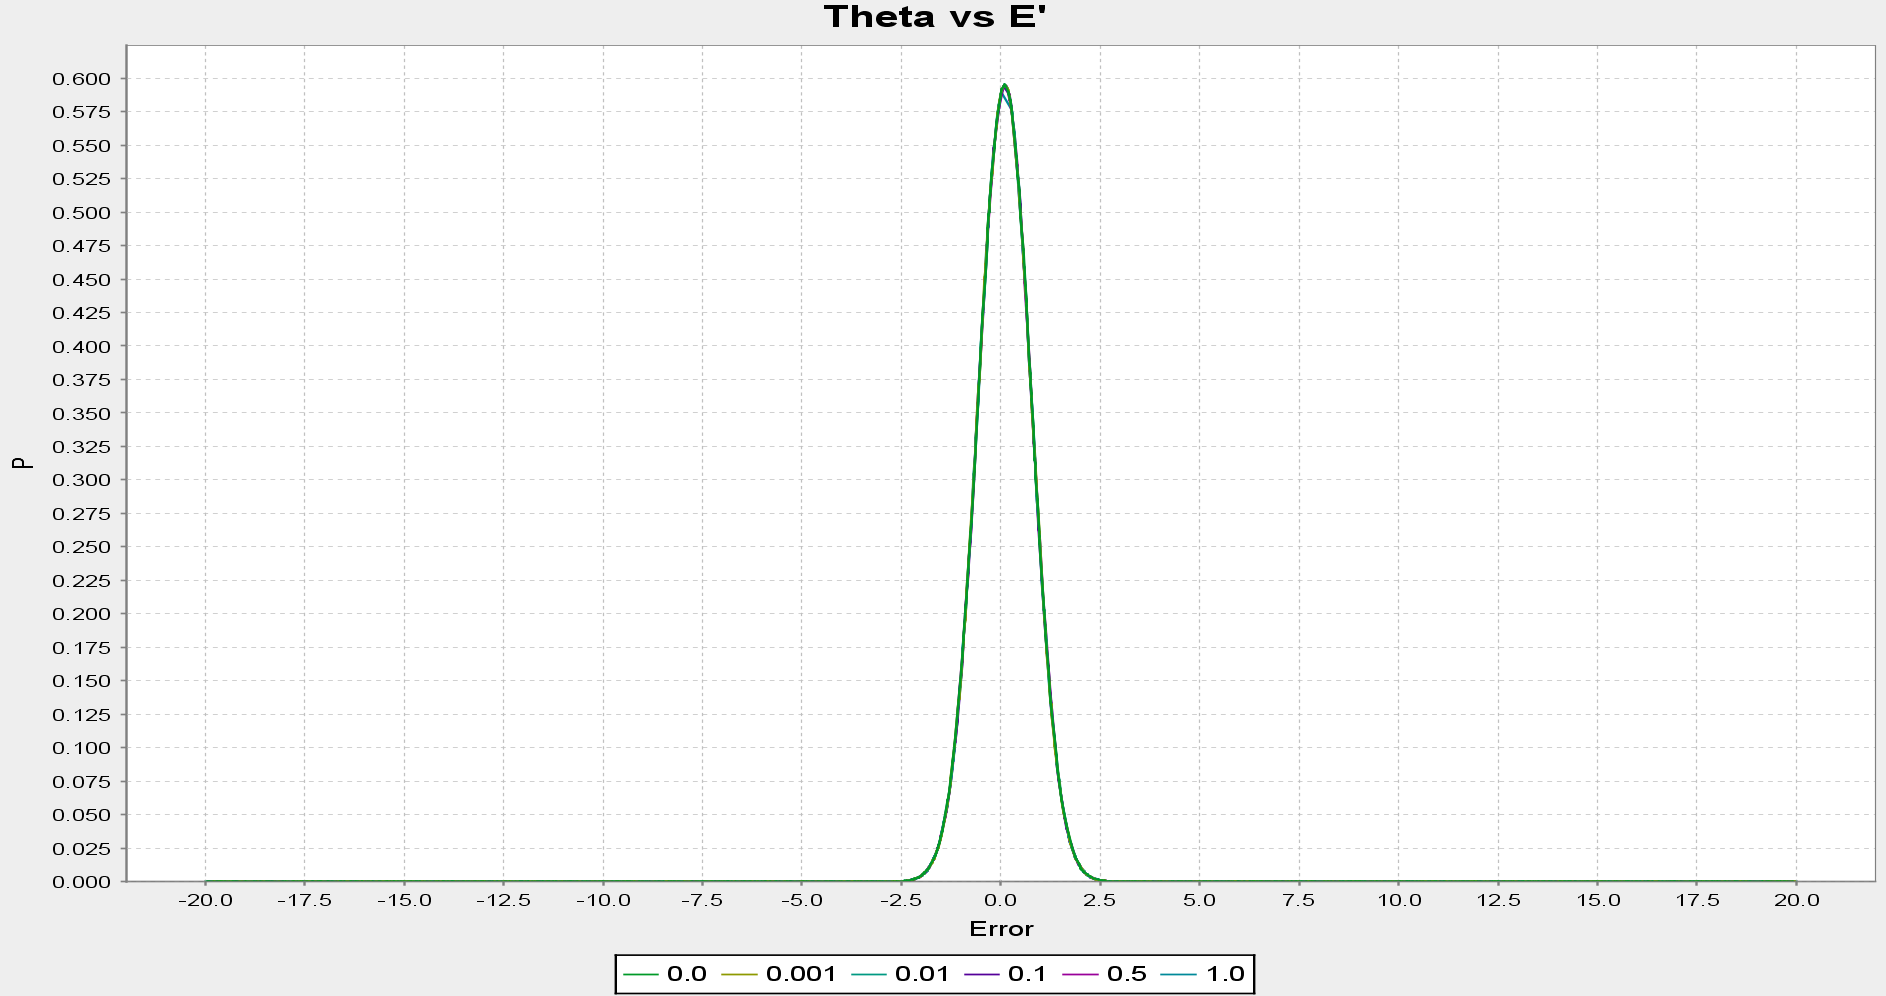
\includegraphics[scale=0.3]{ThetaEDASH}}
\end{figure}

\begin{figure}[H]
\caption{Concentrator Model PDF (Error $e$)}
\label{fig:thetae}
\centerline{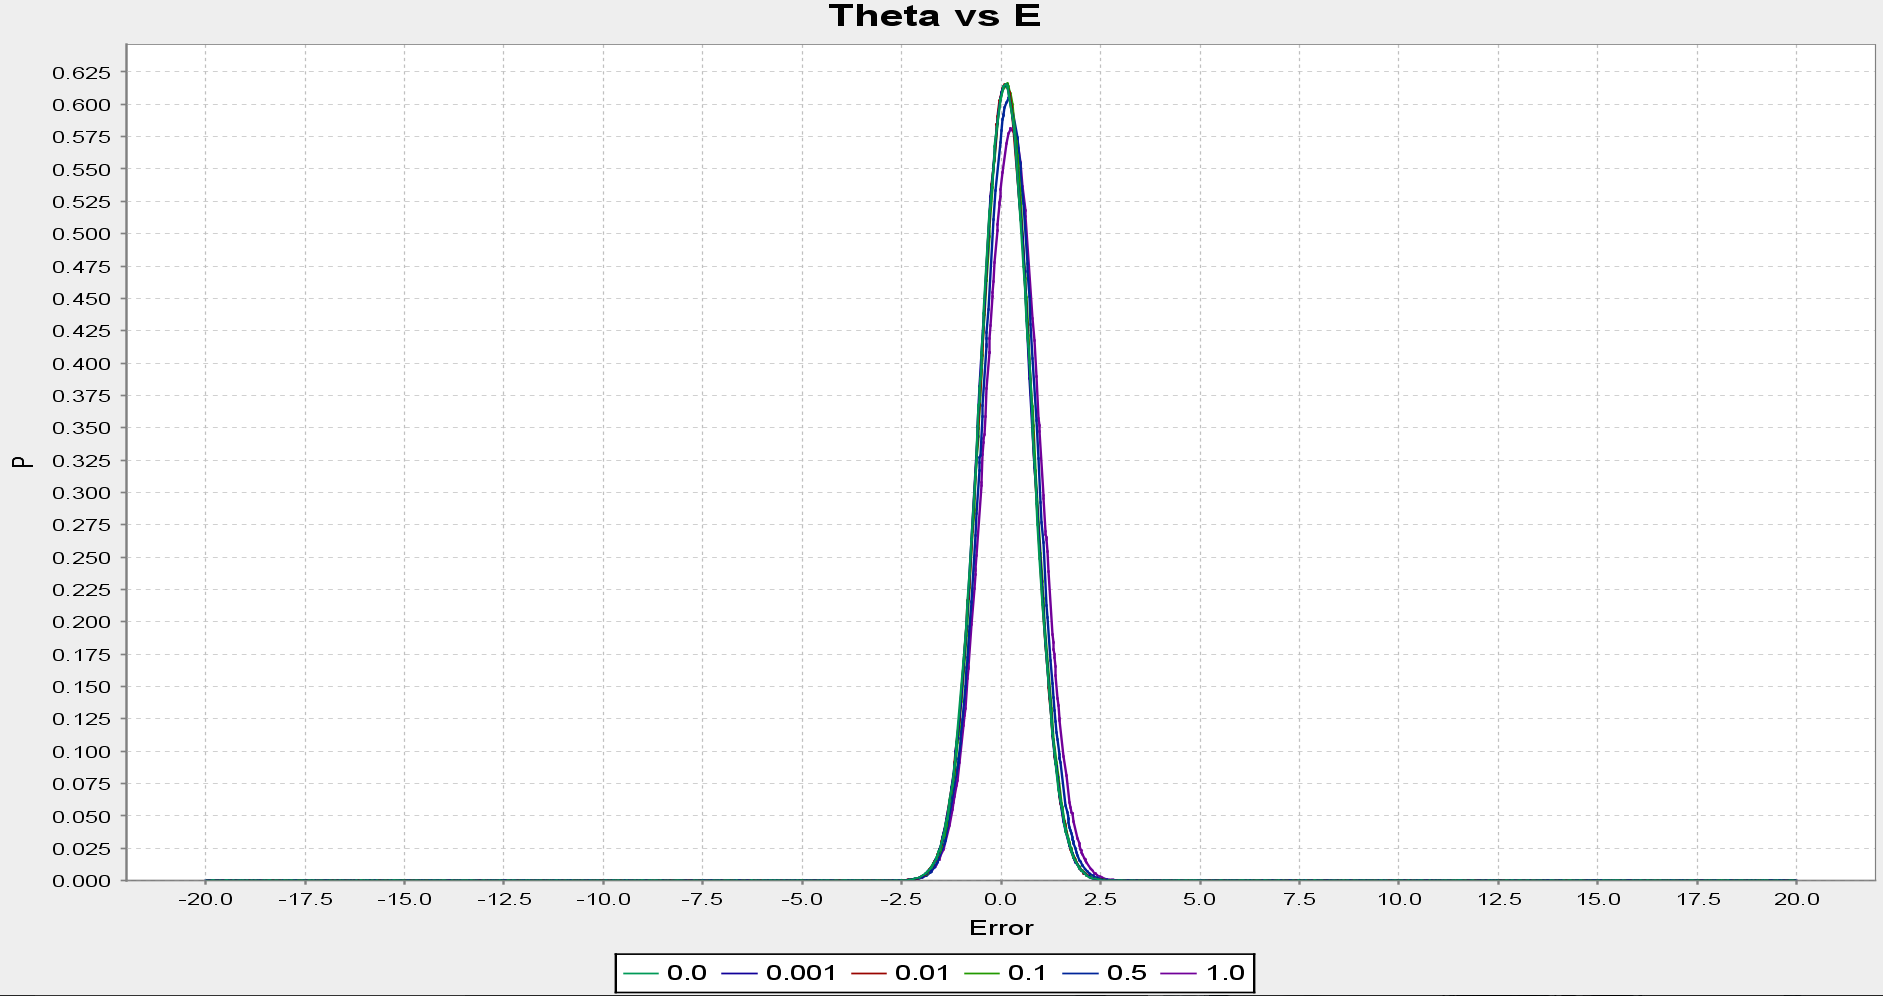
\includegraphics[scale=0.3]{ThetaE}}
\end{figure}

Figures \ref{fig:thetaedash} and \ref{fig:thetae} show the local and concentrator probability density functions respectively as we increase $THETA$. One notices that the mean of the concentrator shifts to the right (increases from 0) as we increase $THETA$ meaning that the error increases. Figure \ref{fig:kldiv} shows the Kullback-Leibler Divergence which is a measure of the difference between the 2 probability distribution functions. In fact as $THETA$ increases the difference increases. The reason there is a slight difference at $THETA=0$, even though they should be identical, is because the system does not update the concentrator model with a worse local model.

\begin{figure}[H]
\caption{$Concentrator - Local$ Model KL-Divergence}
\label{fig:kldiv}
\centerline{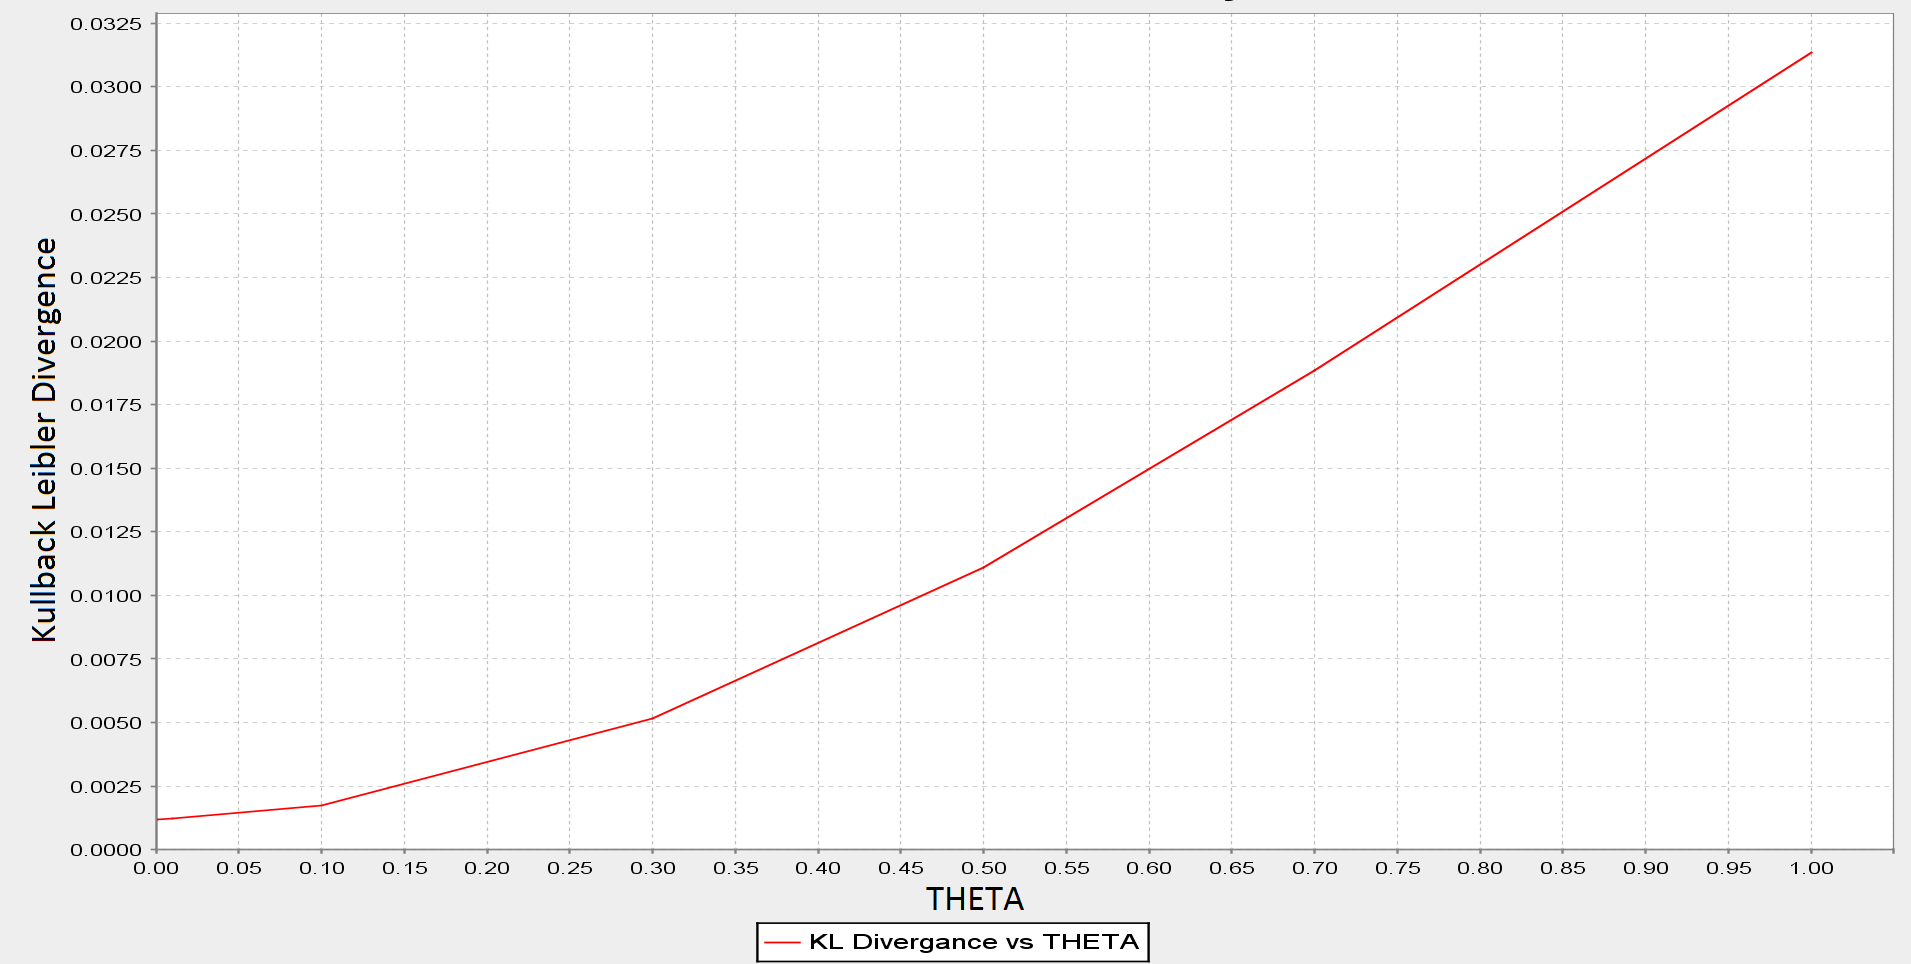
\includegraphics[scale=0.4]{kldivergence}}
\end{figure}

\section{Query Accuracy Evaluation}

In the previous section, we demonstrated how our system gains network efficiency at the expense of a discrepancy error between local and concentrator models. This error value does not depict the full story due to the fact that IoT systems are queried at a concentrator level rather than at device level. When data from several models (nodes) is aggregated together the error might be reduced as all these models contain distributed knowledge about the environment. Thus, from all the data set we randomly select queries and use them to query the concentrator after it finishes learning. This test simulates the typical usage of an IoT system. It lets us study the effect of transmitting fewer messages on the query accuracy. Furthermore, in the implementation chapter we included 2 variables which will directly affect the query accuracy. These are; the $K$ number of clusters (centroids) per device, and the number of models chosen at the concentrator for prediction (Defined as $KNN$ in section \ref{sec:queryAnalytics}).

As a result of this, we will be running tests changing these 2 variable and $Theta$. For each test, the following algorithms (described in the implementation chapter) are used to predict the result of the query. Algorithms:

\begin{itemize}
\item Base Line - (Naive model, most expensive algorithm) All data is transmitted to the concentrator and a single model is built.
\item Ideal - Since this is a test scenario we know from which sensor the query is taken. Only the model for that sensor is used to predict the result.
\item Average - All the models stored in the concentrator are used to calculate the mean.
\item Distance - The closest $K$ models are used to calculate the result. (section \ref{sec:ensembleLearning})
\item Reliability factor - The first $K$ models with the highest weight are used to calculate the result. (section \ref{sec:reliabilityVariable})
\end{itemize}

Figures \ref{fig:0.0}, \ref{fig:0.001}, \ref{fig:0.01}, \ref{fig:0.1}, \ref{fig:0.5}, \ref{fig:1.0} demonstrate our results from these tests. They are 3D graphs, with the x-axis being the KNN, z-axis the K (clusters) and y-axis the error. The different colors show the algorithm used for that particular result. 

\begin{figure}[H]
\caption{$THETA=0.0$ (99.98\% messages)}
\label{fig:0.0}
\centerline{\includegraphics[scale=0.7]{{{0.0}}}}
\end{figure}

\begin{figure}[H]
\caption{$THETA=0.001$ (84.7\% messages)}
\label{fig:0.001}
\centerline{\includegraphics[scale=0.7]{{{0.001}}}}
\end{figure}

\begin{figure}[H]
\caption{$THETA=0.01$ (62.3\% messages)}
\label{fig:0.01}
\centerline{\includegraphics[scale=0.7]{{{0.01}}}}
\end{figure}

\begin{figure}[H]
\caption{$THETA=0.1$ (26.7\% messages)}
\label{fig:0.1}
\centerline{\includegraphics[scale=0.7]{{{0.1}}}}
\end{figure}

\begin{figure}[H]
\caption{$THETA=0.5$ (8.1\% messages)}
\label{fig:0.5}
\centerline{\includegraphics[scale=0.7]{{{0.5}}}}
\end{figure}

\begin{figure}[H]
\caption{$THETA=1.0$ (3.7\% messages)}
\label{fig:1.0}
\centerline{\includegraphics[scale=0.7]{{{1.0}}}}
\end{figure}

From these graphs, we can draw a number of conclusions. Firstly, the \texttt{ideal} algorithm seems to perform the worst on average. This means that using the correct sensor only leads to a high error. On the other hand when we naively take the \texttt{average} of all sensors we get much less error. This implies that knowledge is distributed amongst all the sensors and an optimal subset of sensors should exist to get the least amount of error. The \texttt{baseline} demonstrates the scenario where we have access to 100\% of the data and in fact, produces the lowest error in most cases. Although one notices that as we increase $THETA$ each algorithm approaches the baseline and in some cases we surpass it. This is due to the fact that with a large $THETA$ the model inside the concentrator only captures the essential information and is much more general than the local models.

We introduced the \texttt{distance} and \texttt{reliability factor} algorithms which in contrast to the other algorithms only use a small subset of the models defined by the $KNN$. If $KNN$ is equal to the number of clusters, then the predicted result would be equal to the \texttt{average}. An important thing to note is that $KNN$ seems to be a more important factor to accuracy rather than the number of clusters. $KNN$ is the variable which defines the number of models to choose for averaging at the concentrator level. If $KNN=1$, then only the first model is chosen. So, assuming that the algorithm we have in place always returns the ideal sensor, we will approach the \texttt{ideal} plane instead of the \texttt{baseline} plane.

The predicted result from a very small $KNN$ will be heavily biased and in fact as one can see from the graphs the error is much higher than the average. From these results, we found that the ideal sensor does not produce the least error. Thus, we should have a high $KNN$ but at the same time less than the number of clusters so as to be able to choose a subset of the models, and not all models.

A high number of clusters for each device enables the concentrator to know more about the underlying data. One has to keep in mind that for every cluster, each device has to transmit more bits which would decrease the network efficiency. From these graphs, we observe that with 5 clusters for each device we are able to approach the \texttt{baseline} using the \texttt{reliability factor} algorithm. Increasing $KNN$ does not impact network efficiency as everything would have been already stored on the concentrator at this stage. We also noticed that the distance algorithm seems to produce a more stable set of errors.

\section{Network Efficiency}
\label{sec:networkefficiency}
In this section, we examine whether our system achieves efficient knowledge forwarding at the expense of data accuracy. We compare our system against a simple model which forwards all the data. To evaluate the efficiency we adopt the mica2 \cite{mica2} model. Mica2 operates with a pair of AA batteries that approximately supply 2200 mAh with effective average voltage 3V. The energy costs for a single CPU instruction and transmitting/receiving costs are defined in table \ref{table:energy}.

 \begin{table}[!ht]
 \centering
 \begin{tabular}{||c | c||}
 \hline
 Node Operation Mode & Energy Cost \\
 \hline\hline
 Instruction Execution & 4 nJ/Instruction \\ 
 \hline
 Idle - Stand by & 9.6 mJ/s - 0.33 mJ/s\\
 \hline
 Transmitting - Receiving & 720 nJ/bit - 110 nJ/bit\\
 \hline
\end{tabular}
\caption{Mica2 Energy Costs}
 \label{table:energy} 
\end{table}

\subsection{Average}
In addition to the data, the packet header for each message is 24 bytes. Table \ref{table:thetaMessages} shows the percentage of messages sent when compared to the simple model. As $THETA$ increases the number of messages is reduced but this increases the discrepancy in the model between the concentrator and sensors. When querying the concentrator and using the average method the system uses all the models to predict the result. Thus, there is no need to transfer any other knowledge apart from the regression weights. For each message, our model makes use of 3 weights, while the simple model uses 3 raw values. This implies that each message is equal in size for both systems, and the only difference in energy consumption is the extra computation needed in the sensors.

\begin{table}[!ht]
 \centering
 \begin{tabular}{||c | c | c||}
 \hline
 Algorithm & Messages & Messages \%\\
 \hline\hline
 Simple Model & 111101 & 100\%\\ 
 \hline
 THETA 0.001 & 94142 & 84.7\%\\
 \hline
 THETA 0.01 & 69282 & 62.3\%\\
 \hline
 THETA 0.1 & 29704 & 26.7\%\\
 \hline
 THETA 1.0 & 4126 & 3.7\%\\
 \hline
\end{tabular}
\caption{Theta Messages}
 \label{table:thetaMessages} 
\end{table}

As shown in table \ref{table:energy}, the cost for computation is 180 times less. Our algorithm has 1 instruction for each weight, which adds up to 3 instructions. Then it calculates both the local error and concentrator error, adding another 2 instructions. Thus, for the Average algorithm, which doesn't make use of clustering we have a total of 5 instructions.

We will not be considering the message size in this calculation since in both models they are identical. The sensors in the simple model consume a total of 720nJ * 111,101 messages = 79,992,720 nJ. The concentrator consumes 111,101 messages * 110 nJ = 12,221,110 nJ.
Taking for instance THETA 0.01 the sensors consume 720 nJ * 69,282 messages = 49,883,040 nJ. We include the computation cost which is 4 nJ * 5 instructions * 111,101 messages = 2,222,020 nJ. The concentrator consumes 69,282 messages * 110 nJ = 7,621,020 nJ.

Summing everything up our algorithm uses 59,726,080 nJ while the simple model algorithm uses 92,213,830 nJ, which is 35\% less power consumption. Even though we include the computation costs, transmitting 37.7\% less messages results in an improvement of 35\% power efficiency. This is because our algorithm takes advantage of the fact that transmitting messages is 180 times greater than the energy cost of an instruction. The percentage of messages transmitted can be altered by changing the THETA value according the system's needs. Using the same procedure to calculate the cost for each $THETA$ we get figure \ref{fig:updateModelJoules} which shows the network overhead as the discrepancy error increases.

\begin{figure}[H]
\caption{Network Update Model vs Baseline}
\label{fig:updateModelJoules}
\centerline{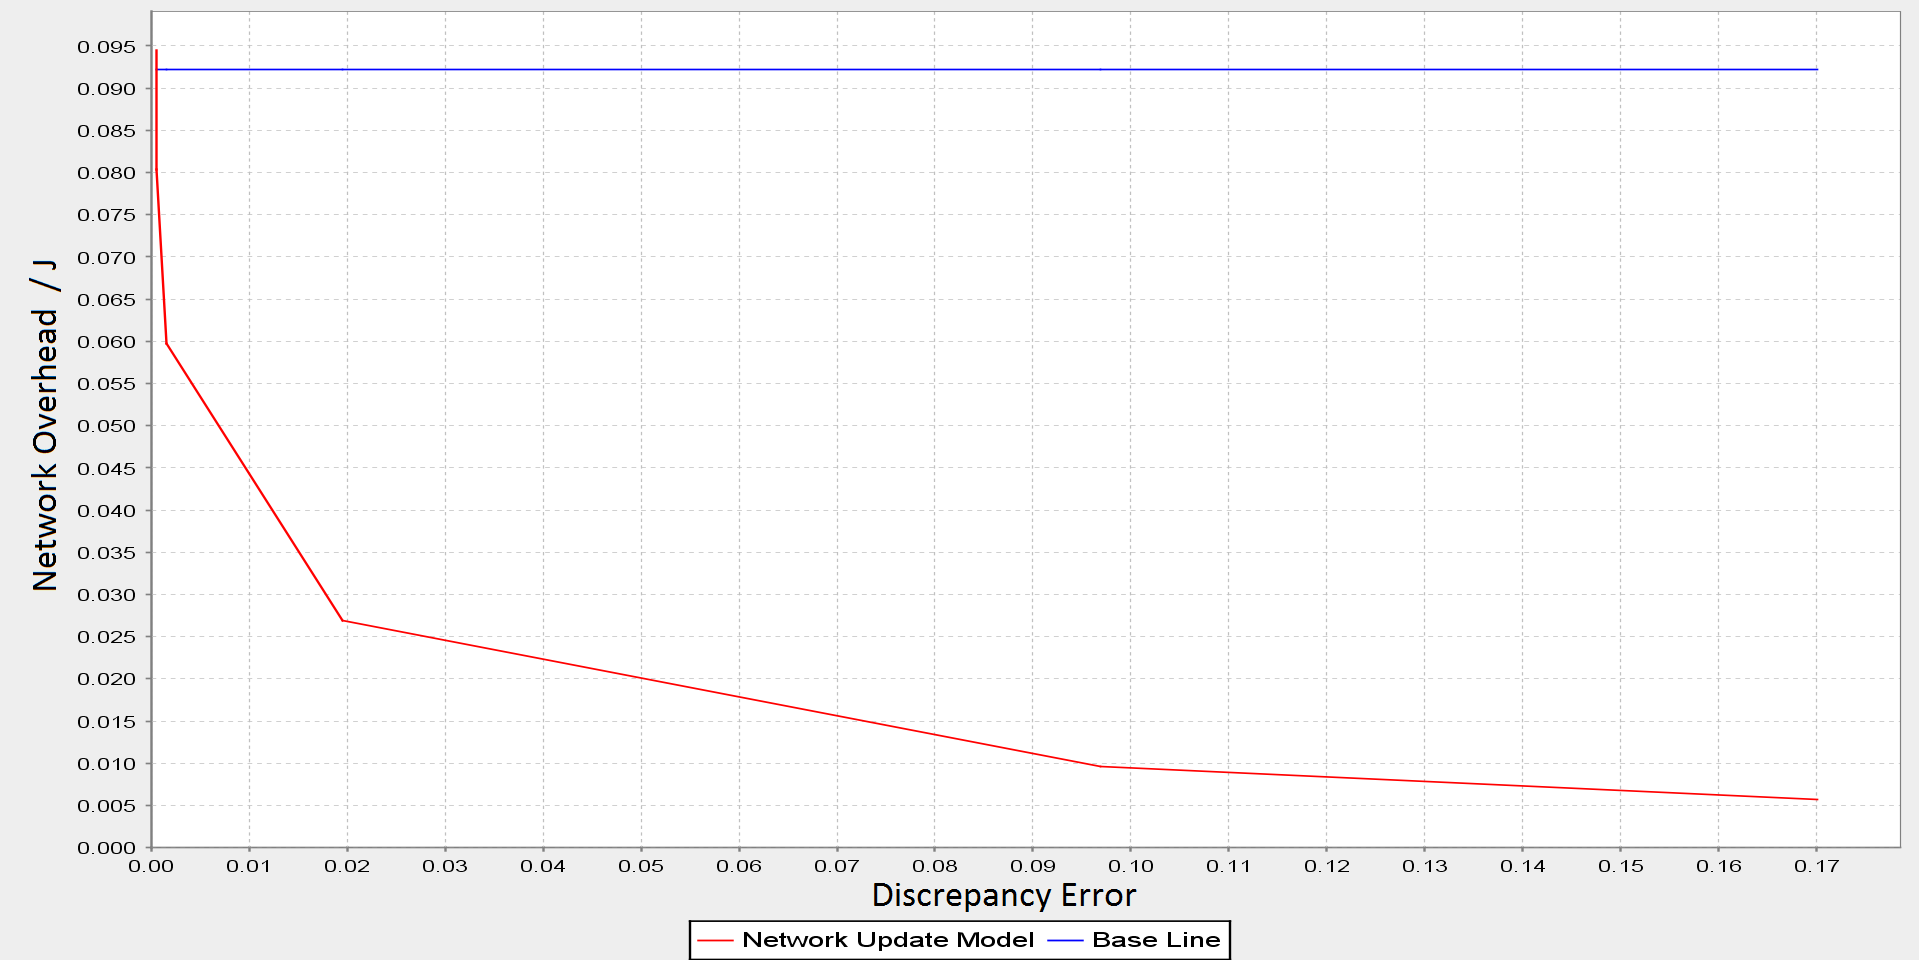
\includegraphics[scale=0.45]{updateModelJoules}}
\end{figure}

\subsection{Including Reliability}
To use our reliability algorithm, the clusters, $errors$ and $used$ values need to be transferred along with the regression models. We introduce an error threshold $GAMMA$ to evaluate the frequency of cluster updates on the accuracy. As an optimization the pairs of $errors$ and $used$ values can be multiplied together before transmission and sent as 1 value instead of 2. Using $K=3$ centroids, we have 6 values (each centroid has $(x,y)$) and 3 other values representing the $errors$ and $used$ counters. The message that contains only the regression model consists of 3 values but when adding the quantized information it adds up to a total of 12 values. This is 4 times larger than the simple model message, thus $GAMMA$ should be adjusted so as to achieve network efficiency.

\begin{table}[!ht]
 \centering
 \begin{tabular}{|| c | c | c | c ||}
 \hline
 Algorithm & Messages (3 values) & Messages (12 values)\\
 \hline\hline
 Simple Model & 111101 & 0 \\ 
 \hline
 GAMMA 0 & 0 & 69282 \\
 \hline
 GAMMA 0.1 & 52476 & 16806 \\
 \hline
 GAMMA 1.0 & 68331 & 951 \\
 \hline
\end{tabular}
\caption{$THETA$ $0.01$, $K=3$, $GAMMA$ Message Distribution}
 \label{table:thetaGammaMessages} 
\end{table}

Table \ref{table:thetaGammaMessages} lists the number of messages that are sent with and without the clusters for $THETA$ $0.01$. $GAMMA$ 1.0 drastically reduces the number of time clusters are sent. Figure \ref{fig:gammak3} is a plot of each algorithm using $THETA$ $0.01$ at $GAMMA$ 0, 0.1 and 1.0. Increasing $GAMMA$ does not seem to increase the error for the reliability algorithm, which means the same information can be transferred with less energy. 

\begin{figure}[H]
\caption{$THETA$ $0.01$, $K=3$, $GAMMA$ Error plot}
\label{fig:gammak3}
\centerline{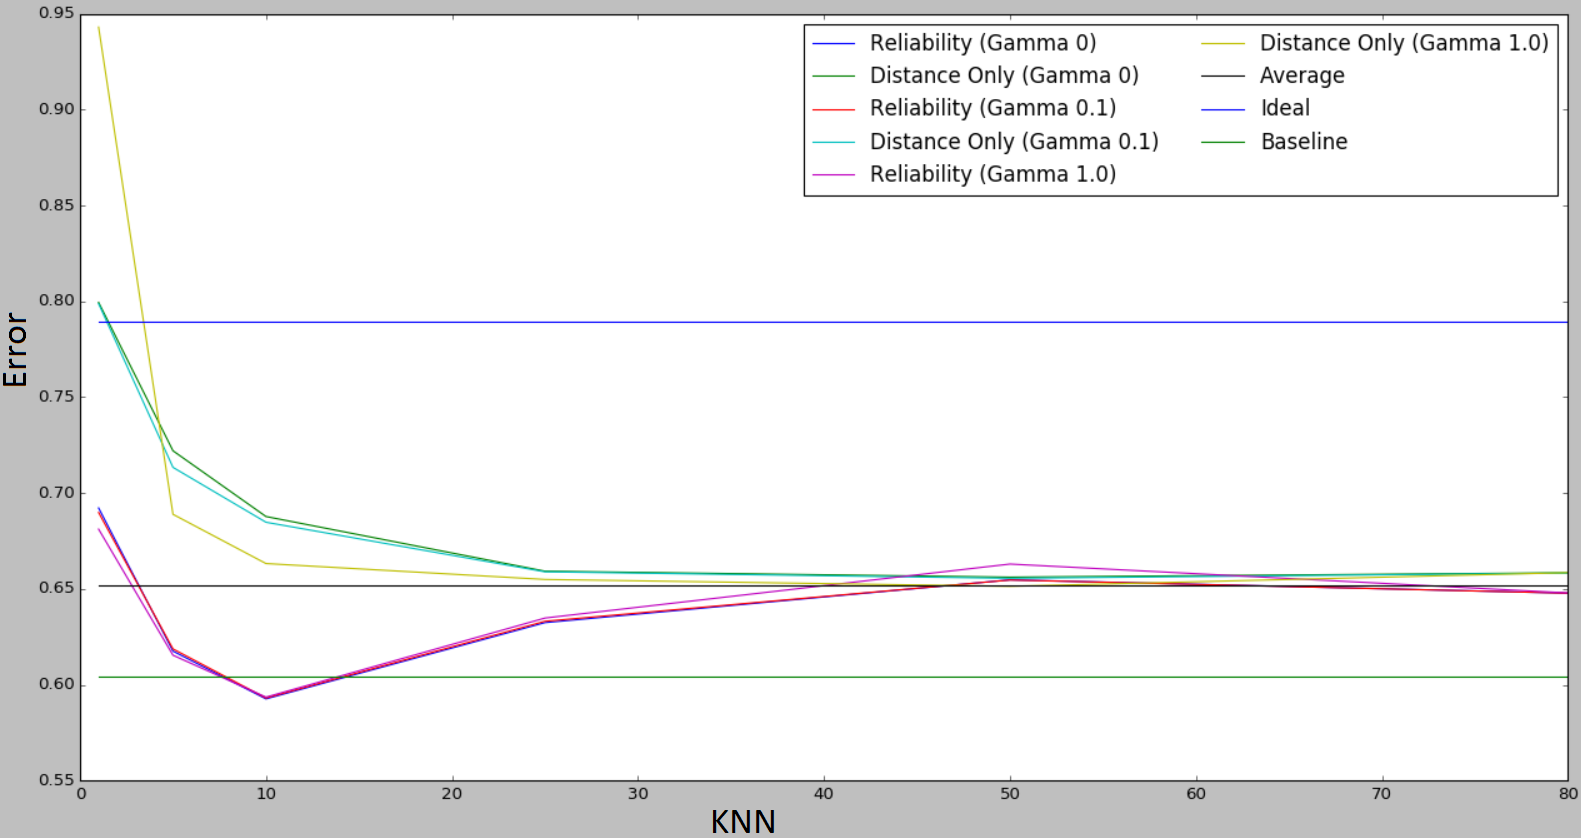
\includegraphics[scale=0.5]{k3gamma}}
\end{figure}

Using the information of all $THETA$ figure \ref{fig:ensembleModelJoules} is generated. It represents the trade-off in accuracy vs the network overhead due to ensemble learning (reliability algorithm). The energy calculations used previously for the Average algorithm were tweaked to include the larger messages and extra computations. Using this algorithm an extra 4 instructions are needed (1 to find the closest cluster, 1 update for each K). Adding the previous 5 instructions from the learning model we get a total of 9 instructions. 

\begin{figure}[H]
\caption{Ensemble Model (K=3, KNN=10) vs Baseline}
\label{fig:ensembleModelJoules}
\centerline{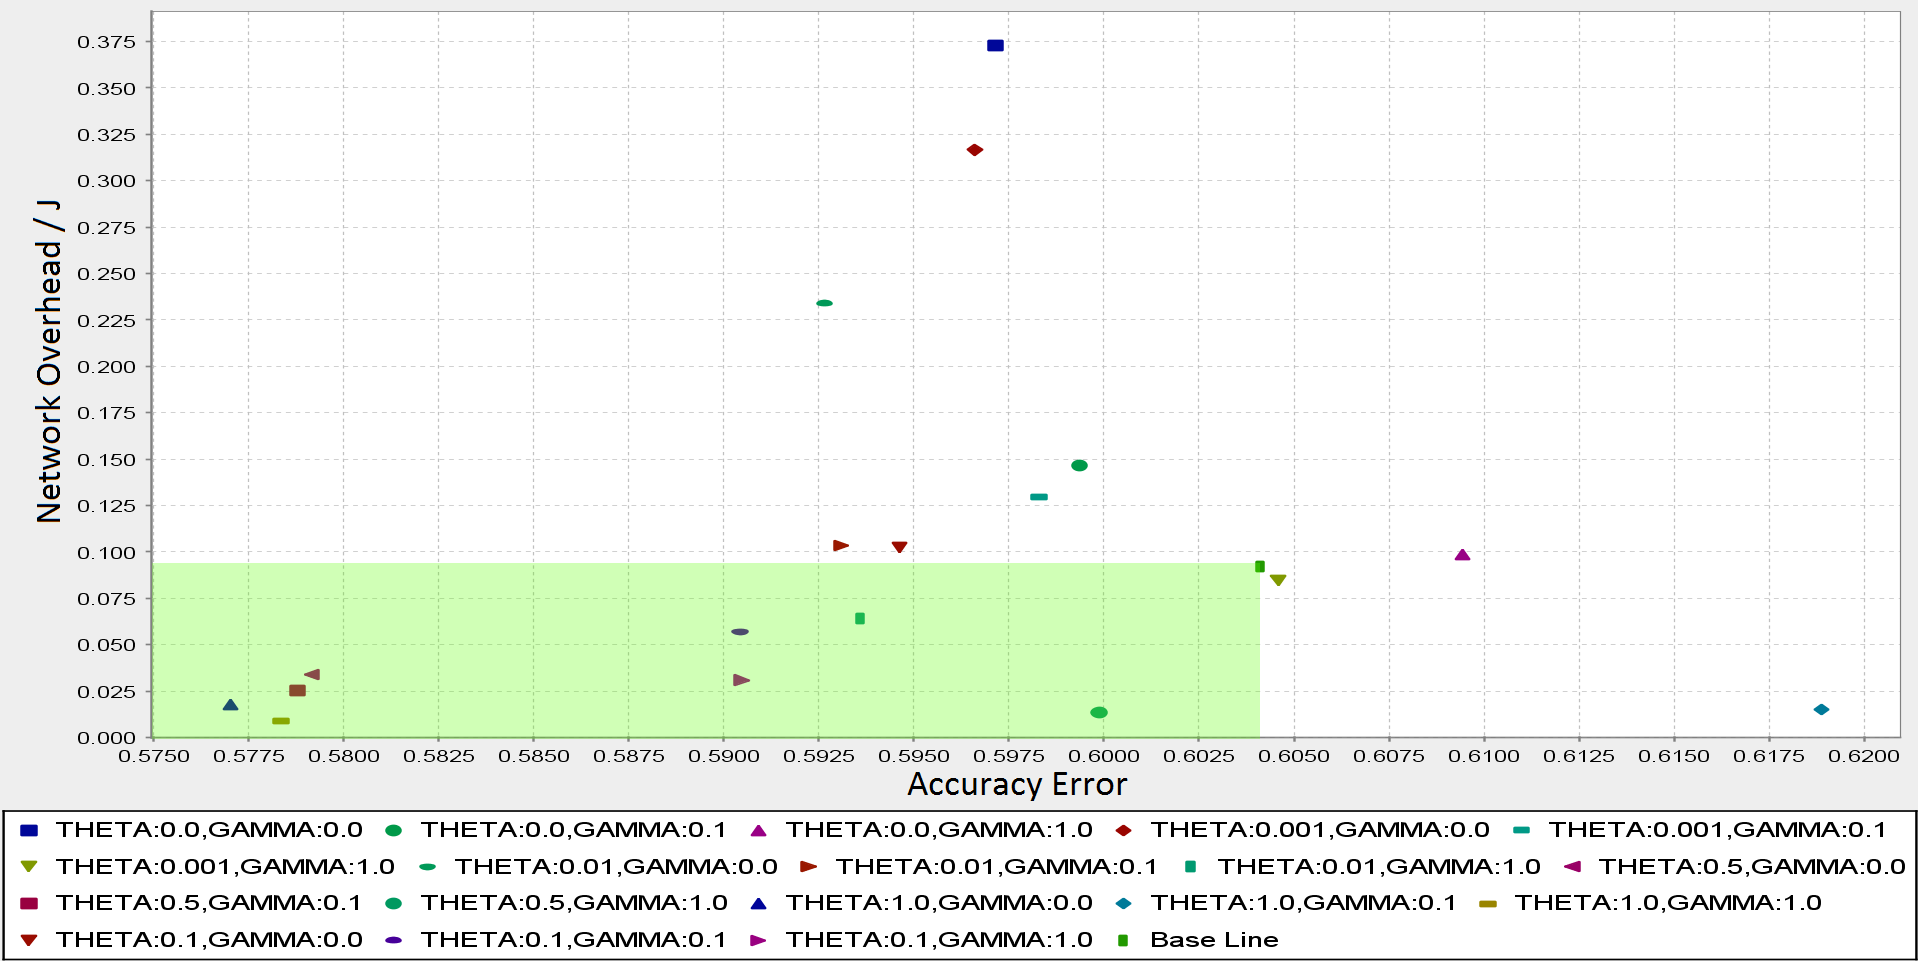
\includegraphics[scale=0.45]{ensembleModelJoules}}
\end{figure}

The green overlay on figure \ref{fig:ensembleModelJoules} shows the configurations which result in better accuracy and more power efficiency than the baseline.

\chapter{Conclusion}
The primary motivation for undertaking this work was to analyse and investigate algorithms for improving the network efficiency in wireless networks while simultaneously diffuse knowledge among the network. In this final chapter, we discuss the principal contributions of this work and comment on how they coincide with the project aims. Finally, we identify opportunities for future work and describe how one might go about to achieve them.

\section{Achievements}
In this work, we investigated algorithms on how to promote network efficiency in wireless sensor networks and reduce query accuracy error at the concentrator. Our main contributions are listed below:
\begin{itemize}
\item A system capable of simulating a real-life IoT environment. This includes the gathering of statistics from multiple sensors and a concentrator.
\item Compared our regression model with the simple model and evaluated the network efficiency gain.
\item Evaluated the extended regression model which quantizes the input with the aim of achieving better query accuracy.
\item A case study of our algorithms based on the Beijing U-Air dataset\cite{air-quality-inference-meets-big-data} and Mica2\cite{adaptiveDataForwarding} sensors.
\end{itemize}

\section{Future Work}
Although the contributions of our work are precisely what we set out to achieve, there are several other approaches and extensions which could be explored in greater depth under less strict time constraints.

\paragraph{Non-Linear Regression:}In our work, we only considered linear regression as the learning model inside the sensors, but non-linear regression can instead be used to better represent the underlying data. 
\paragraph{History of Models:}In the evaluation chapter, we observed better query accuracy as we increased $THETA$. Thus, this would suggest that we can store a history of models instead of just one model for each sensor at the concentrator.
\paragraph{Concentrator teaching:}In our algorithm, we were transmitting the $error$ and $used$ values along with the centroids to indicate which are the most reliable centroids. An alternative approach would be to occasionally transmit raw data to the concentrator. This raw data at the concentrator can be used to quantize the input space and teach the concentrator which subset of models to use in various circumstances.

\section{Final Remarks}
Whilst we recognize that the algorithms created and described in this work can be further enhanced, these should serve as a point of reference for further research in this field of study. Furthermore, through our work, we demonstrated the importance and feasibility of using distributed statistical learning and knowledge diffusion for improving network efficiency in wireless sensor networks.

\bibliographystyle{plain}
\bibliography{mproj}
\end{document}
